\documentclass[10pt]{article}
\usepackage[utf8]{inputenc}
\usepackage{empheq}
\usepackage[inline, shortlabels]{enumitem}
\usepackage{gensymb}
\usepackage{multicol}
\setlength{\parskip}{0.5cm plus4mm minus3mm}
\setlength{\parindent}{0pt}
\usepackage{amsmath}
\usepackage{esint}
\usepackage{upgreek}
\usepackage[margin=0.6in]{geometry}
 \geometry{
 left=12mm,
 bottom=20mm
 }
\usepackage{amssymb}
\usepackage{cs170}
\usepackage{graphicx}
\usepackage{scrextend}


\begin{document}
\date{}
\title{\vspace{-5ex} \dunhd{Math 53: Multivariable Calculus Notes} \vspace{-5ex}}
\maketitle
\begin{multicols}{2}
\section{Parametric Curves, Polar Coordinates}
\begin{enumerate}
    \item \textbf{Parametric Equations} 
    \begin{enumerate}
         \item Some curves cannot be expressed in the form $y=f(x)$ or $x=f(y)$. We can instead express $x$ and $y$ as functions of a third variable $t$, called a \textbf{parameter.} The \textbf{parametric equations} $x = f(t)$ and $y=g(t)$ trace out a curve as $t$ varies. If we restrict $a \leq t \leq b$, then the curve has initial point $(f(a), g(a))$ and terminal point $(f(b), g(b))$.
         
         \item Note that familiar functions $y=f(x)$ can be written in parametric form as $x=t$ and $y=f(t)$. We can attempt to eliminate the parameter $t$ to recover a Cartesian equation of the curve.
         
         \item For example, the parametric equations $x = a\cos{t}$, $y = b\sin{t}$, $0 \leq t \leq 2\pi$ sketch out the ellipse $\frac{x^2}{a^2} + \frac{y^2}{b^2}=1$ in a counterclockwise direction.
         
         \item The curve traced out by a point on the circumference of a circle as the circle rolls along a straight line is called a \textbf{cycloid}. For a circle of radius $r$ with starting point on the origin, the cycloid is given by $x = r( \theta - \sin{\theta})$ and $y = r(1 - \cos{\theta})$ for $\theta \in \mathbb{R}$; one arch is $0 \leq \theta \leq 2\pi$.
    \end{enumerate}
    
    \item \textbf{Calculus of Parametric Curves}
    \begin{enumerate}
        \item \textbf{Derivatives:} By the chain rule, for $dx / dt \neq 0$,
        \begin{align*}
            \frac{dy}{dx} = \frac{dy / dt}{dx / dt}
        \end{align*}
        
        \item \textbf{Second derivatives:} 
        \begin{align*}
            \frac{d^2y}{dx^2} = \frac{\frac{d}{dt}(\frac{dy}{dx})}{\frac{dx}{dt}}
        \end{align*}
        \item In computing tangents, recall point-slope form of a line: $y - y_1 = m(x - x_1)$.  
        \item Horizontal tangents occur when the numerator is 0; vertical tangents occur when the denominator is 0; L'Hospitals rule may help when both the numerator and denominator are 0.
        
        \item \textbf{Areas:} If a curve is sketched out by parametric equations $x = f(t)$ and $y = g(t)$, $\alpha \leq t \leq \beta$, then the area under the curve is 
        \begin{align*}
            A = \int_a^b y \, dx = \int_\alpha^\beta g(t) f'(t) \, dt
        \end{align*}
        where $a = f(\alpha)$ and $b = f(\beta)$. There is an analogous formula when integrating with respect to $y$:
        \begin{align*}
            A = \int_c^d x \, dy = \int_\alpha^\beta g'(t) f(t) \, dt
        \end{align*}
        where $c = g(\alpha)$ and $d = g(\beta)$.
        \item \textbf{Arc length:} If a curve $C$ is described by the parametric equations $x = f(t)$ and $y = g(t)$, $\alpha \leq t \leq \beta$, where $f'$ and $g'$ are continuous on $[\alpha, \beta]$, and $C$ is traversed exactly once as $t$ increases from $\alpha$ to $\beta$, then the length of $C$ is 
        \begin{align*}
            L = \int_\alpha^\beta \sqrt{ \left(\frac{dx}{dt}\right)^2 + \left(\frac{dy}{dt}\right)^2} \, dt
        \end{align*}
        \item \textbf{Surface Area:} Suppose a curve $C$ is described by the parametric equations $x = f(t)$ and $y = g(t)$, $\alpha \leq t \leq \beta$, where $f'$ and $g'$ are continuous on $[\alpha, \beta]$, $g(t) \geq 0$, and $C$ is traversed exactly once as $t$ increases from $\alpha$ to $\beta$. If $C$ is rotated about an axis, the area of the resulting surface is         \begin{align*}
            &S = \int_\alpha^\beta 2\pi y \, ds &\text{rotation about x-axis} \\
            &S = \int_\alpha^\beta 2\pi x \, ds &\text{rotation about y-axis}
        \end{align*}
        where
        \begin{align*}
            ds = \sqrt{ \left(\frac{dx}{dt}\right)^2 + \left(\frac{dy}{dt}\right)^2} \, dt
        \end{align*}
    \end{enumerate}
    
    \item \textbf{Polar Coordinates}
    \begin{enumerate}
        \item The \textbf{polar coordinate system} can be more convenient than Cartesian coordinates for some purposes. There exists a \textbf{pole} $O$, or origin, and a ray starting at $O$ called the \textbf{polar axis}. 
        \item Every point $P$ has coordinates $(r, \theta)$, where $r$ is the distance from $P$ to $O$ and $\theta$ is the angle between the polar axis and the line $OP$. Note that $(0, \theta)$ represents $O$ for any angle $\theta$. 
        \item We use the convention that $(-r, \theta)$ is the point $(r, \theta + \pi)$.
        \item The relationship between polar and Cartesian coordinates is given by
        \begin{align*}
            x = r \cos{\theta} \hspace{6mm} y = r \sin{\theta} \\
            r^2 = x^2 + y^2 \hspace{6mm} \tan{\theta} = \frac{y}{x}
        \end{align*}
        \item The graph of a polar equation $r = f(\theta)$ consists of all points that have a polar representation $(r, \theta)$ whose coordinates satisfy the equation. In sketching a polar curve, it is sometimes helpful to graph $r=f(\theta)$ in Cartesian coordinates to read off values of $r$ as $\theta$ increases.
        \item A polar curve can be converted into Cartesian coordinates by manipulating the equation into groups of $r\cos{}$ and $r\sin{}$ terms, and substituting $x$ and $y$ into them, respectively.
        \item If the polar equation is unchanged when $\theta$ is replaced with $-\theta$, the curve is symmetric about the polar axis.
        \item $r=\sin{\theta}$ is a circle with radius $\frac{1}{2}$ and center $(0,\frac{1}{2})$, while $r=\cos{\theta}$ is a circle with radius $\frac{1}{2}$ and center $(\frac{1}{2},0)$. The graphs of $r=\sin{c\theta}$ and $r=\cos{c\theta}$ both look like flowers with $c$ petals if $c$ is odd and flowers with $2c$ petals if $c$ is even.
        \item \textbf{Derivatives:} For $r=f(\theta)$, regard $\theta$ as a parameter to get $x = f(\theta)\cos{\theta}$ and $y = f(\theta)\sin{\theta}$. Then
        \begin{align*}
            \frac{dy}{dx} = \frac{dy / d\theta}{dx / d\theta} = \frac{f'(\theta)\sin{\theta} + f(\theta)\cos{\theta}}{f'(\theta)\cos{\theta} - f(\theta)\sin{\theta}}
        \end{align*}
        
        \item \textbf{Areas:} The area of a region whose boundary is given by a polar equation $r=f(\theta)$:
        \begin{align*}
            A = \frac{1}{2} \int_a^b f(\theta)^2 \, d\theta
        \end{align*}
        
        The area of the region bounded above by $f(\theta)$ and below by $g(\theta)$ is
        \begin{align*}
            A = \frac{1}{2} \int_a^b (f(\theta)^2 - g(\theta)^2) \, d\theta
        \end{align*}
        
        \item \textbf{Arc Length:} The length of a curve with polar equation $r=f(\theta)$, $a \leq \theta \leq b$ is
        \begin{align*}
            L = \int_a^b \sqrt{f(\theta)^2 + \left( \frac{dr}{d\theta} \right)^2} \, d\theta
        \end{align*}
    \end{enumerate}
\end{enumerate}


\section{Vectors and the Geometry of Space}
\begin{enumerate}
    \item \textbf{Three-Dimensional Coordinates}
    \begin{enumerate}
        \item In two-dimensional geometry, the graph of an equation involving $x$ and $y$ is a curve in $\mathbb{R}^2$. In three-dimensional geometry, an equation in $x,y,z$ is a \textbf{surface} in $\mathbb{R}^3$.

        
        \item The distance between two points in three dimensions is $\sqrt{\Delta x^2 + \Delta y^2 + \Delta z^2}$.
        \item The equation of a sphere with center $C(h,k,l)$ and radius $r$ is 
        \begin{align*}
            (x-h)^2 + (y-k)^2 + (z-l)^2 = r^2
        \end{align*}
    \end{enumerate}
    \item \textbf{Vectors (in $\mathbb{R}^n$)}
    \begin{enumerate}
        \item Note we we will use the notation $\langle a_1, \hdots, a_n \rangle$ to denote a vector in $\mathbb{R}^n$ (not an inner product).
        \item Parallelogram Law: If $\vec{u}$ and $\vec{v}$ are vectors positioned so that the initial point of $\vec{v}$ is at the terminal point of $\vec{u}$, then $\vec{v} + \vec{u}$ is the vector from the initial point of $\vec{u}$ to the terminal point of $\vec{v}$.
        \item The \textbf{magnitude} of vector $\vec{v} = \langle a_1, a_2, a_3 \rangle$ is the length: 
        \begin{align*}
            \| \vec{v} \| = \sqrt{a_1^2 + a_2^2 + a_3^2}
        \end{align*}
        \item The standard basis vectors of $\mathbb{R}^3$:
        \begin{align*}
            \vec{i} = \langle 1,0,0 \rangle \hspace{5mm} 
            \vec{j} = \langle 0,1,0 \rangle \hspace{5mm} 
            \vec{k} = \langle 0,0,1 \rangle 
        \end{align*}
        Sometimes vectors are written as linear combinations of $\vec{i},\vec{j},\vec{k}$.
        % \item The distance between vectors $\vec{v}$ and $\vec{u}$ is $\| \vec{v} - \vec{u} \|$.
    \item The \textbf{dot product} (the standard inner product) of vectors $\vec{u}$ and $\vec{v}$ $\in$ $\mathbb{R}^n$ is defined as:
    \begin{equation*}
       \vec{u} \cdot \vec{v} = u_1v_1+\ldots u_nv_n
    \end{equation*}
    Properties:
    \begin{align*}
        \vec{u} \cdot \vec{v} = \vec{v} \cdot \vec{u} \\
        (c\vec{u}) \cdot \vec{v} = c(\vec{u} \cdot \vec{v}) \\
        (\vec{u} + \vec{x}) \cdot \vec{v} = \vec{u} \cdot \vec{v} + \vec{x} \cdot \vec{v}
    \end{align*}
    If $\theta$ is the angle between $\vec{v}$ and $\vec{u}$, we have
    \begin{equation*}
        \vec{u} \cdot \vec{v} = \| \vec{u} \| \hspace{.5mm} \| \vec{v} \| \cos{\theta}
    \end{equation*}
    Two vectors $\vec{u}$ and $\vec{v}$ are \textbf{orthogonal} iff $\vec{u} \cdot \vec{v} = 0$.
    \item The projection of a vector $\vec{y}$ onto another vector $\vec{x}$ is given by
    \begin{align*}
        \text{proj}_{\vec{x}} \vec{y} = \frac{\vec{x} \cdot \vec{y}}{\| \vec{x} \|^2}\vec{x}
    \end{align*}
    The scalar projection of $\vec{y}$ onto $\vec{x}$ is given by
    \begin{align*}
        \text{comp}_{\vec{x}} \vec{y} = \frac{\vec{x} \cdot \vec{y}}{\| \vec{x} \|}
    \end{align*}
    
    \item The \textbf{cross product} of $\vec{u}$ and $\vec{v}$, denoted $\vec{u} \times \vec{v}$, is given by the determinant:
    \begin{align*}
        \vec{u} \times \vec{v} = 
        \begin{vmatrix}
        \vec{i} & \vec{j} & \vec{k} \\
        u_1 & u_2 & u_3 \\
        v_1 & v_2 & v_3 
        \end{vmatrix}
    \end{align*}
    $\vec{u} \times \vec{v}$ is orthogonal to both $\vec{u}$ and $\vec{v}$. Properties:
    \begin{align*}
        \vec{u} \times \vec{v} = -\vec{v} \times \vec{u} \\
        (c\vec{u}) \times \vec{v} = c(\vec{u} \times \vec{v}) = \vec{u} \times (c\vec{v}) \\
        (\vec{u} + \vec{v}) \times \vec{z} = \vec{u} \times \vec{z} + \vec{v} \times \vec{z}
    \end{align*}
    \item If $\theta$ is the angle between $\vec{u}$ and $\vec{v}$, we have
    \begin{equation*}
        \| \vec{u} \times \vec{v} \| = \| \vec{u} \| \hspace{.5mm} \| \vec{v} \| \sin{\theta}
    \end{equation*}
    Thus $\vec{u} \times \vec{v} = \vec{0}$ iff $\vec{u}$ and $\vec{v}$ are parallel. We can interpret $\| \vec{u} \times \vec{v} \|$ as the area of the parallelogram determined by $\vec{u}$ and $\vec{v}$.
    \item The product $\vec{u} \cdot (\vec{v} \times \vec{z})$ is known as the \textbf{scalar triple product} of vectors $\vec{u}, \vec{v}, \vec{z}$:
    \begin{align*}
        \vec{u} \cdot (\vec{v} \times \vec{z}) = 
        \begin{vmatrix}
        u_1 & u_2 & u_3 \\
        v_1 & v_2 & v_3 \\
        z_1 & z_2 & z_3
        \end{vmatrix}
    \end{align*}
    The volume of the parallelepiped determined by the vectors $\vec{u}, \vec{v}, \vec{z}$ is $\| \vec{u} \cdot (\vec{v} \times \vec{z}) \|$.
    \end{enumerate}

\item \textbf{Equations of Lines and Planes}
\begin{enumerate}
    \item An equation of the line through the point $(x_0, y_0, z_0)$ parallel to the direction vector $\vec{v} = \langle a, b, c \rangle$ is $\vec{r} = \vec{r_0} + t\vec{v}$. In parametric form,
    \begin{align*}
        x = x_0 + at \hspace{6mm}
        y = y_0 + bt \hspace{6mm}
        z = z_0 + ct
    \end{align*}
    
    \item \textbf{Skew lines} are lines in 3D space that are not parallel and do not intersect. Lines are parallel if their corresponding direction vectors are proportional. Lines intersect if there exist values of $t$ and $s$ such that $x,y,z$ parameters are all equal.
    
    \item A \textbf{plane} in space is completely determined by a point and a vector orthogonal to the plane. 
    \item A scalar equation of the plane through $P_0(x_0, y_0, z_0)$ with normal vector $\vec{n} = \langle a,b,c \rangle$ is 
    \begin{align*}
        a(x-x_0) + b(y-y_0) + c(z-z_0) = 0
    \end{align*}
    We can collect terms to obtain a linear equation of the form $ax+by+cz+d=0$, where $\langle a,b,c \rangle$ is the normal vector.
    \item To find the plane passing through points $P,Q,R$, we can find $\vec{PQ}$ and $\vec{PR}$ to obtain two vectors on the plane (recall the vector from $A$ to $B$ is $B-A$). Take their cross product to obtain a normal vector.
    \item Two planes are parallel if their normal vectors are parallel. If they are not, then they intersect. 
    \item To find the line of intersection between two planes, find a point on that line (e.g., take $z=0$ and solve for $x,y$) and take the cross product of the normal vectors to obtain a direction vector of the line. 
    \item The angle between planes is given by the acute angle between their normal vectors.
    \item The distance between the point $P_1(x_1,y_1,z_1)$ and the plane $ax+by+cz+d=0$ is the scalar projection of $P_1$ onto the normal vector of the plane:
    \begin{align*}
        D = \frac{|ax_1 + by_1+cz_1+d|}{\sqrt{a^2+b^2+c^2}}
    \end{align*}
\end{enumerate}

\item \textbf{Quadric Surfaces}
\begin{enumerate}
    \item A \textbf{quadric} surface is the graph of a degree-2 equation in $x,y,z$. If one of the variables is missing, the surface is cylindrical.
    % \item Review of 2D Conic sections:
    % \begin{itemize}
    %     \item An upward opening parabola is of the form $y=x^2$.
    %     \item An ellipse is of the form $\frac{x^2}{a^2} + \frac{y^2}{b^2} = 1$.
    %     \item A hyperbola with foci on the x-axis is of the form $\frac{x^2}{a^2} - \frac{y^2}{b^2} = 1$. Reversing the roles of $x$ and $y$ result in a hyperbola with foci on the y-axis.
    %     \vspace{-2mm}
    % \begin{align*}
    %     \hspace{-8mm}
    %     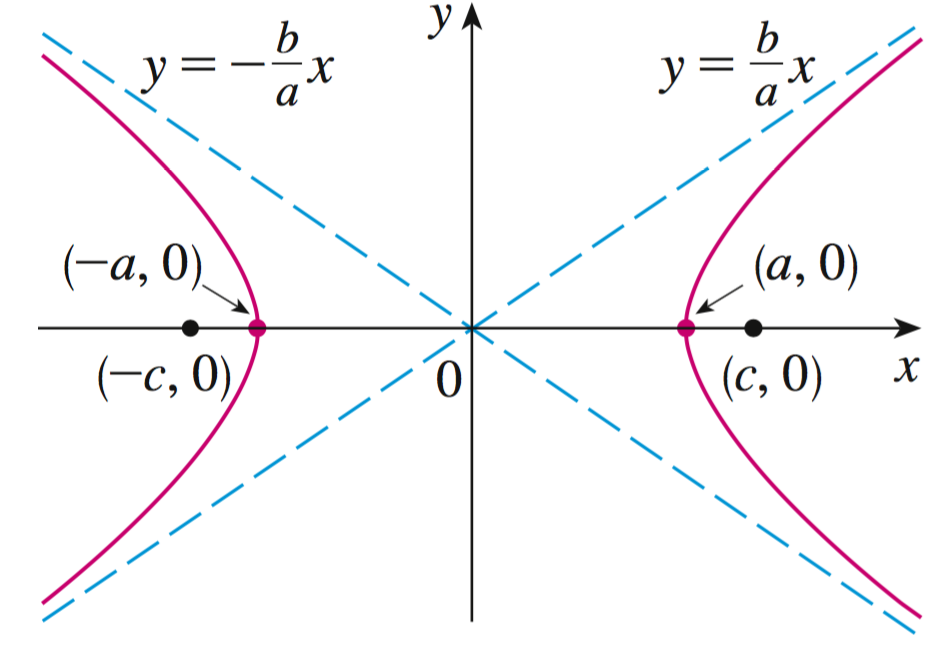
\includegraphics[width=3cm]{hyperbola.png} \hspace{10mm} 
    %     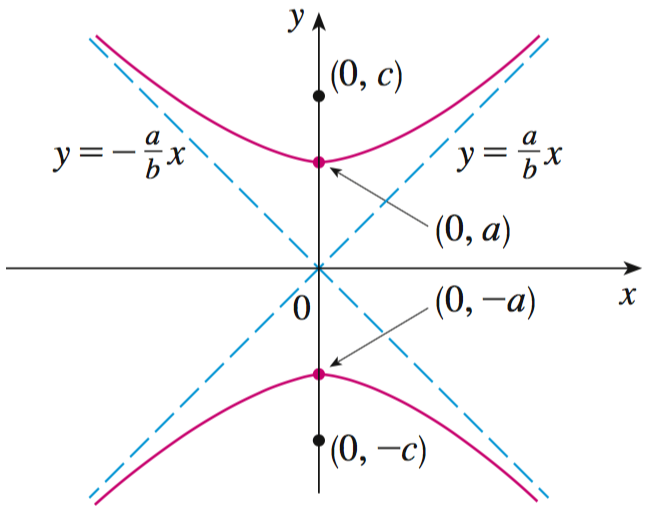
\includegraphics[width=3cm]{hyperbola2.png}
    % \end{align*}
    % \end{itemize}
    
    \begin{align*}
    \hspace{-3mm}
        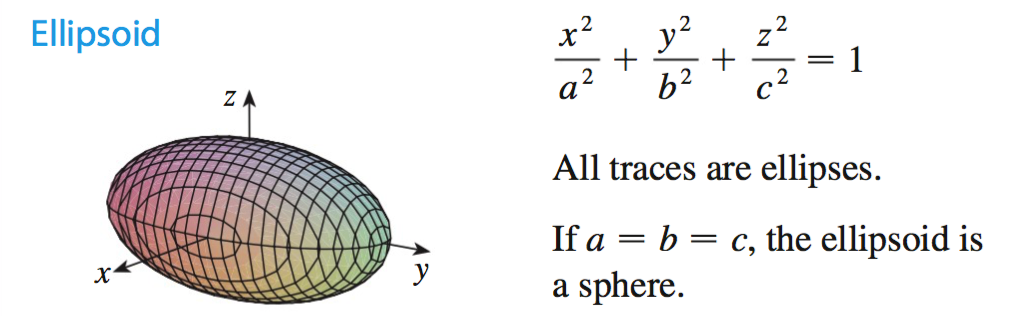
\includegraphics[width=8cm]{ellip.png} \\
        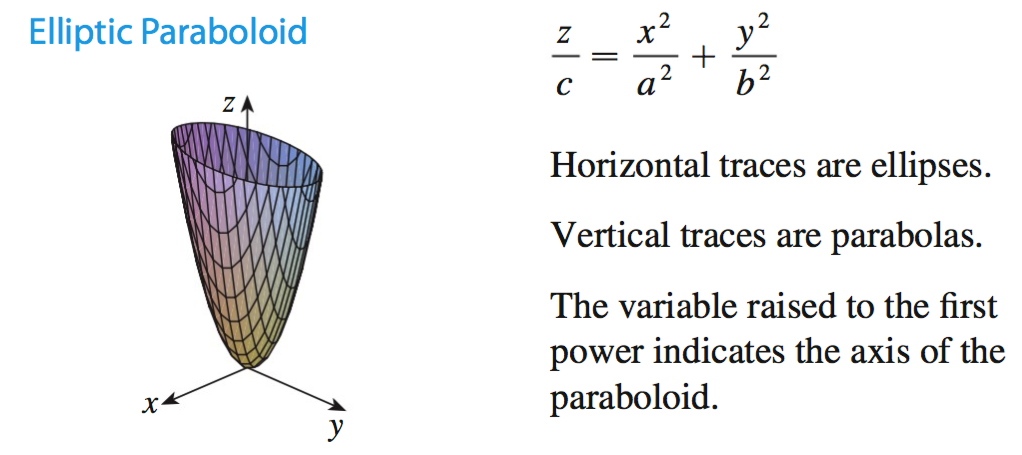
\includegraphics[width=8cm]{eparab.png} \\
        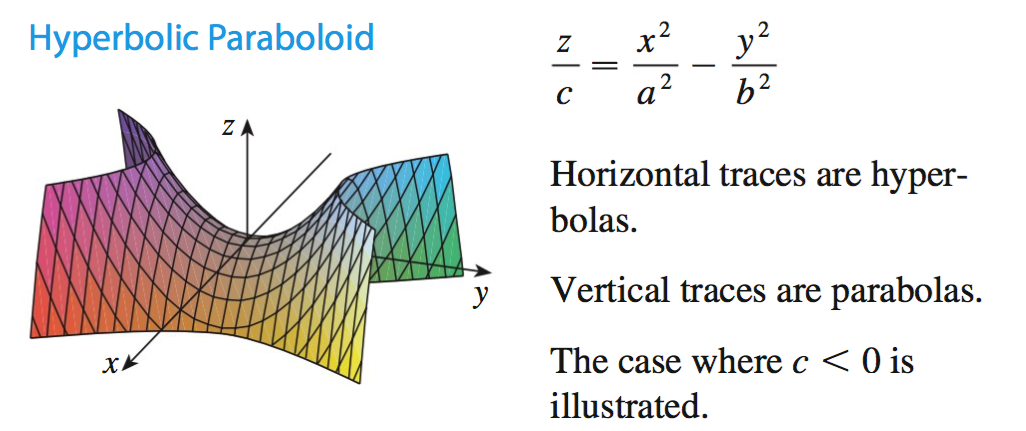
\includegraphics[width=8cm]{hyperp.png} \\
        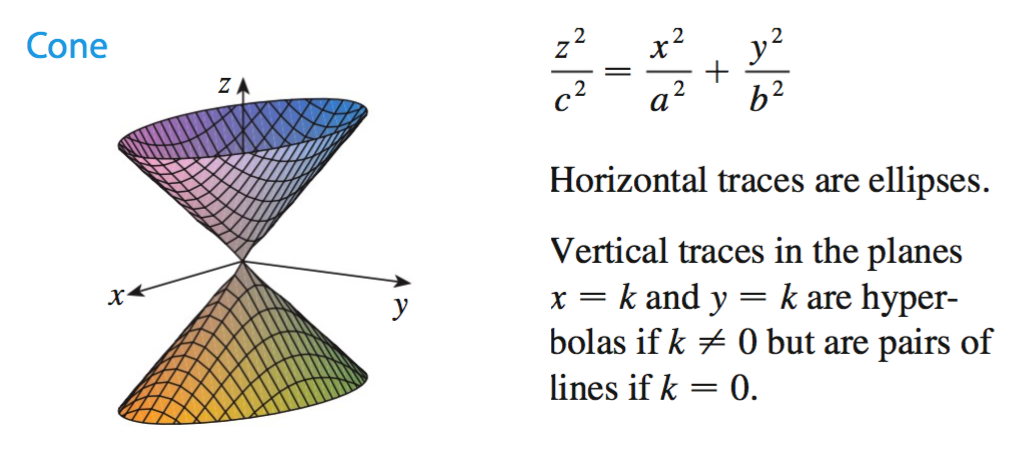
\includegraphics[width=8cm]{cone.png} \\
        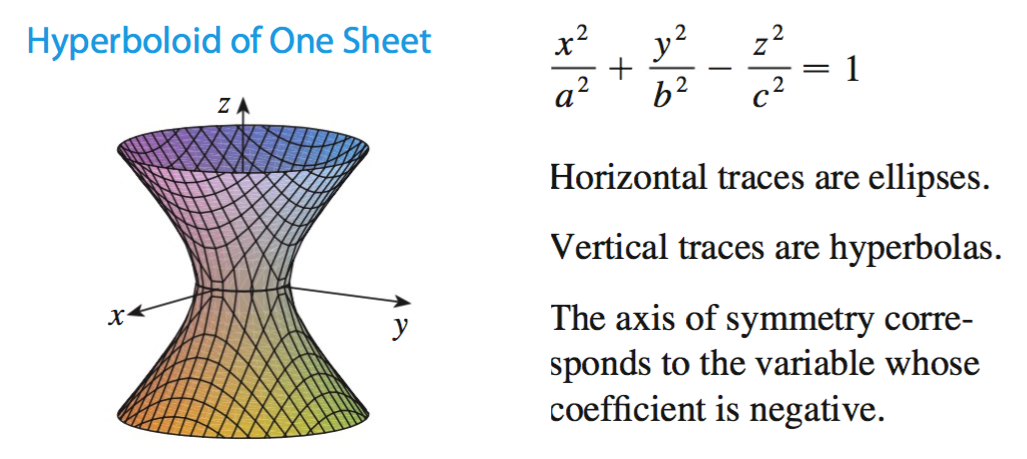
\includegraphics[width=8cm]{hyper1.png} \\
        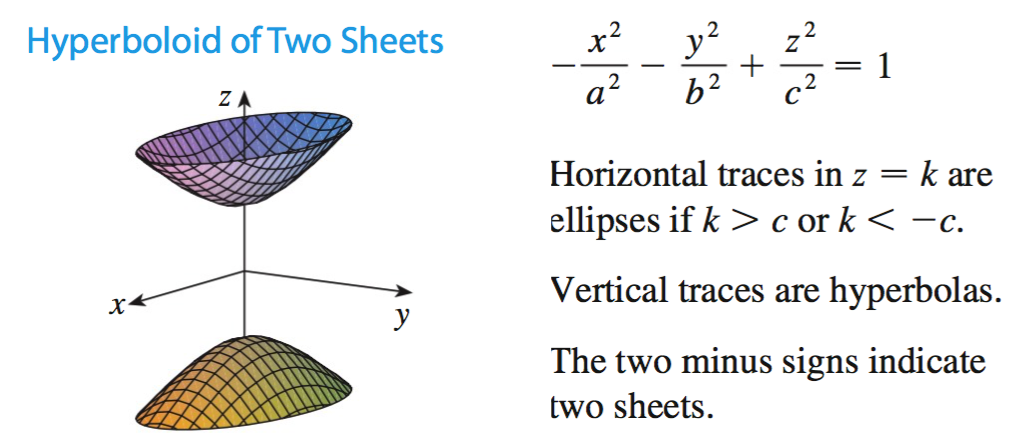
\includegraphics[width=8cm]{hyper2.png}
    \end{align*}
    
    \item To sketch the graph of a surface, it is helpful to draw \textbf{traces}, or cross-sections parallel to the coordinate planes (take $x,y$ or $z$ to be 0 and consider the resulting shape).
\end{enumerate}
\end{enumerate}
\section{Vector Functions}
\begin{enumerate}
    \item \textbf{Vector Functions}
    \begin{enumerate}
        \item A vector-valued function maps real numbers to vectors. We will study functions $\vec{r}: \mathbb{R} \mapsto \mathbb{R}^3$:
        \begin{align*}
            \vec{r}(t) = \langle f(t), g(t), h(t) \rangle
        \end{align*}
        The domain of $\vec{r}$ consists of all values of $t$ for which the component functions are defined. As $t$ varies throughout an interval, $\vec{r}$ defines a \textbf{space curve} traced out by the tip of the vector $\vec{r}(t)$. 
        
        \item We say a space curve given by $\vec{r}(t)$ is \textbf{smooth} if $\vec{r'}$ is continuous and $\vec{r'}(t) \neq \vec{0}$ for all $t$.
        
        \item To determine a vector function for the curve of intersection of two surfaces: Amounts to finding $x,y,z$ such that the equations of two surfaces are satisfied. Try to parametrize a cylinder with two variables (with $\cos$ and $\sin$) and solve for third variable using other equation.
        
        \item Derivatives:
        \begin{align*}
            \vec{r'}(t) = \langle f'(t), g'(t), h'(t) \rangle
        \end{align*}
        The tangent line to a space curve at point $P$ is defined to be the line through $P$ parallel to the tangent vector $\vec{r'}(t)$.
        
        \item More facts about space curves (e.g. arc length) will be explored later with line integrals. 
        
         
    \end{enumerate}
    
    
\end{enumerate}

\section{Partial Derivatives}
\begin{enumerate}
    \item \textbf{Functions of Several Variables}
    \begin{enumerate}
        \item A function $f$ of two variables assigns a real number $f(x,y)$ to each ordered pair $x,y$ from a set $D$, the domain.
        \item The \textbf{level curves} of $f$ are the curves with equations $f(x,y)=k$ for some constant $k$. Sketching level curves at various values of $k$ can help visualize the graph of the function.
    \end{enumerate}
    \item \textbf{Limits}
    \begin{enumerate}
        \item We say that the limit of $f(x,y)$ as $(x,y)$ approaches $(a,b)$ is $L$, written
        \begin{align*}
            \lim_{(x,y) \rightarrow (a,b)} f(x,y) = L
        \end{align*}
        if for every $\epsilon > 0$ there is a corresponding $\delta > 0$ such that if $0 < \sqrt{(x-a)^2 + (y-b)^2} < \delta$ then $|f(x,y) - L| < \epsilon$. In other words, the distance between $f(x,y)$ and $L$ can be made arbitrarily small by making the distance from $(x,y)$ and $(a,b)$ sufficiently small (but not 0).
        
        \item The \textbf{squeeze theorem} can be used to prove a limit exists. If $f(x,y) \leq g(x,y) \leq h(x,y)$  for all $(x,y)$ near $(a,b)$, and $$\lim_{(x,y) \rightarrow (a,b)} f(x,y) = L = \lim_{(x,y) \rightarrow (a,b)} h(x,y)$$ then $$\lim_{(x,y) \rightarrow (a,b)} g(x,y) = L$$ This is done by trapping a subset of the function within a finite range, transforming all sides of the inequality to obtain the original function, then taking the limit of the inequality. Recall that $\lim_{x \rightarrow 0} \frac{sin{x}}{x} = 1$. 
        
        \item If $f(x,y) \rightarrow L_1$ as $(x,y) \rightarrow (a,b)$ along a path $C_1$ and $f(x,y) \rightarrow L_2$ as $(x,y) \rightarrow (a,b)$ along a path $C_2$, where $L_1 \neq L_2$, then $\lim_{(x,y) \rightarrow (a,b)} f(x,y)$ \textit{does not exist}. Some simple paths to try may include $x=a,y=b,$ or $y=mx$.
        
        \item Another method for computing limits is to convert to polar coordinates; take $x=r\cos{\theta}$ and $y=\sin{\theta}$, and $\lim_{(x,y) \rightarrow (0,0)}$ becomes $\lim_{r \rightarrow 0}$. Then apply L’Hospital’s rule.
        
        \item $f(x,y)$ is \textbf{continuous} at $(a,b)$ if $\lim_{(x,y) \rightarrow (a,b)}$ $f(x,y) = f(a,b)$. All polynomials and rational functions (ratios of polynomials) of two variables are continuous \textit{on their domain}, so limits can be found by direct substitution.
    \end{enumerate}
    
    \item \textbf{Partial Derivatives}
    \begin{enumerate}
        \item The \textbf{partial derivative} of $f$ with respect to $x$, denoted $f_x$ or $\partial f / \partial x$, is the derivative of $f$ with all other variables fixed: 
        $$
        \frac{\partial}{\partial x} f(x,y) = f_x(x,y) = \lim_{h\rightarrow 0} \frac{f(x+h,y) - f(x,y)}{h}$$
        \item Implicit differentiation: To compute $\frac{\partial z}{\partial x}$, differentiate implicity with respect to $x$, treating $y$ as a constant.
        \item The notation $f_{xyz}$ means first differentiate with respect to $x$, then $y$, then $z$. By \textbf{Clairaut’s theorem}, if $f_{xy}$ and $f_{yx}$ exist and are continuous on the domain of $f$, then $f_{xy} = f_{yx}$. 
        \item Partial differential equations arise in a wide variety of phenomena in physics. For example, Laplace's equation in three-dimensions is given by
        $$ \frac{\partial^2 u}{\partial x^2} + \frac{\partial^2 u}{\partial y^2} + \frac{\partial^2 u}{\partial z^2} = 0$$
        If $u(x,y,z)$ represents electric or gravitational potential at $(x,y,z)$, then $u$ satisfies Lapace's equation.
    \end{enumerate}
    
    \item \textbf{Tangent Planes and Linear Approximation} 
    \begin{enumerate}
        \item An equation of the tangent plane to the surface $z=f(x,y)$ at the point $P(x_0, y_0, z_0)$ is
        \begin{align*}
            z - z_0 = f_x(x_0, y_0)(x-x_0) + f_y(x_0, y_0)(y-y_0)
        \end{align*}
        \item The tangent plane at point $P$ is the plane that most closely approximates the surface $S$ near $P$. Solving the plane equation for $z$ yields the linearization at $P$, denoted $L(x,y)$.
        \item If the partial derivatives $f_x$ and $f_y$ exist and are continuous at $(a,b)$, then $f$ is \textbf{differentiable} at $(a,b)$.
        
        \item For a differentiable function $z=f(x,y)$, the \textbf{differential} $dz$, defined by 
        $$
        dz = \frac{\partial z}{\partial x} dx + \frac{\partial z}{\partial y} dy
        $$
        represents the change in height of the tangent plane at a particular point when $x$ and $y$ change by an amount $dx$ and $dy$, respectively. $dz$ is an approximation for $\Delta z$ for small changes.
    \end{enumerate}
    
    \item \textbf{The Chain Rule}
    \begin{enumerate}
        \item If $z$ is a function of several variables, which are in turn functions of other variables, then $z$ is a composite function that can be differentiated according to the chain rule.
        \item \textbf{Chain rule:} Suppose $u$ is a differentiable function of $n$ variables $x_1, \hdots, x_n$ and each $x_i$ is a differentiable function of $m$ variables $t_1, \hdots t_m$. Then $u$ is a function of $t_1, \hdots t_m$ and
        \begin{align*}
            \frac{\partial u}{\partial t_i} = \frac{\partial u}{\partial x_1} \frac{\partial x_1}{\partial t_i} + \frac{\partial u}{\partial x_2} \frac{\partial x_2}{\partial t_i} + \hdots + \frac{\partial u}{\partial x_n} \frac{\partial x_n}{\partial t_i} 
        \end{align*}
        \item It is helpful to draw the tree diagram of a function to visualize the chain rule: draw edges to indicate function-of relationships and write the corresponding partial derivative on each branch. Then to compute $\partial z / \partial s$, for example, sum the product of partial derivatives along each path from $z$ to $s$. 
        \begin{align*}
            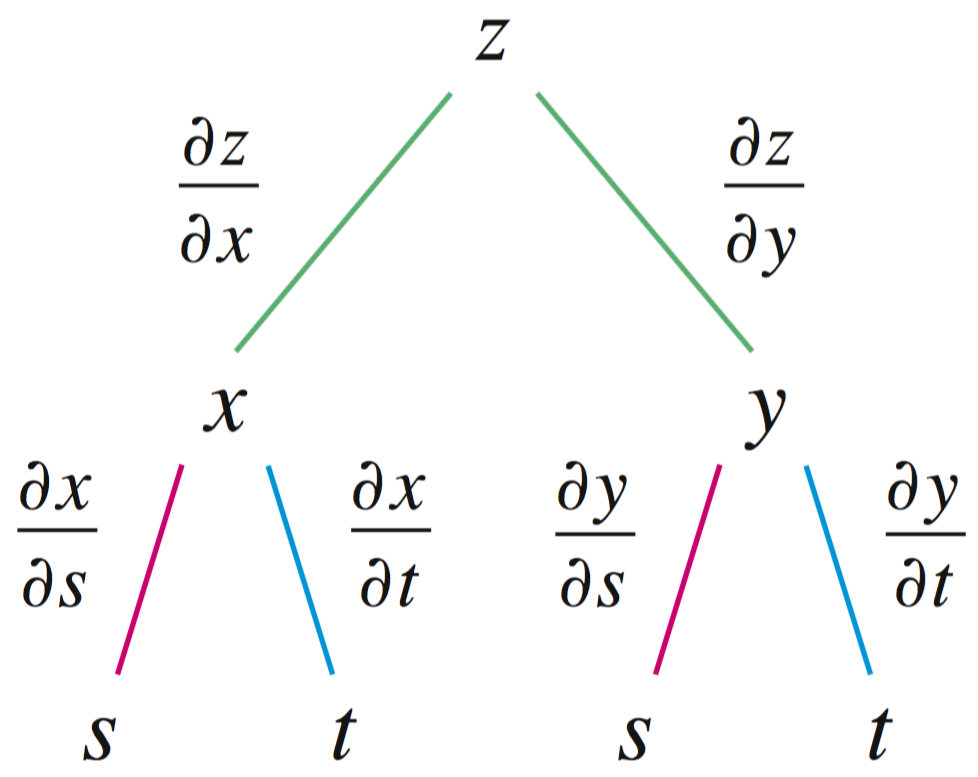
\includegraphics[width=3.8cm]{chain_rule.png}
        \end{align*}
        \item Second order partial derivative example: consider the function described above in the diagram. Then
        \begin{align*}
            \frac{\partial^2 z}{\partial t^2} = \frac{\partial}{\partial t} \left( \frac{\partial z}{\partial x} \frac{\partial x}{\partial t} + \frac{\partial z}{\partial y}\frac{\partial y}{\partial t} \right)
        \end{align*}
        Computing this will involve applications of the product rule and chain rule.
    \end{enumerate}
    \columnbreak
    \item \textbf{Directional Derivatives and Gradients}
    \begin{enumerate}
        \item The partial derivative of $f$ with respect to $x$ yields the rate of change of $f$ in the direction of the $x$-axis. We now consider a new kind of derivative indicating the rate of change in any direction.
        \item The \textbf{directional derivative} of $f$ at $(x, y)$ in the direction of the unit vector $\vec{u} = \langle a,b \rangle$ is
        \begin{align*}
            D_u f(x,y) = \lim_{h \rightarrow 0} \frac{f(x+ha, y+hb) - f(x,y)}{h}
        \end{align*}
        Hence $f_x$ and $f_y$ are just special cases of the directional derivative for $\vec{i}$ and $\vec{j}$, respectively.
        \item If $f$ is a differentiable function of $x$ and $y$, then $f$ has a directional derivative in the direction of any unit vector $\vec{u} = \langle a,b \rangle$ and 
        \begin{align*}
            D_u f(x,y) = f_x(x,y)a + f_y(x,y)b
        \end{align*}
        Note that if $\vec{u}$ makes an angle $\theta$ with the postive $x$-axis, then $\vec{u} =\langle \cos{\theta}, \sin{\theta} \rangle$.
        \item If $f$ is a function of two variables $x$ and $y$, then the \textbf{gradient} of $f$ is the vector function $\nabla f$:
        \begin{align*}
            \nabla f(x,y) = \langle f_x(x,y), f_y(x,y) \rangle = \frac{\partial f}{\partial x} \vec{i} + \frac{\partial f}{\partial y} \vec{j}
        \end{align*}
        Note that $D_u f(x,y) = \nabla f(x,y) \cdot \vec{u}$, i.e., the scalar projection of the gradient vector onto $\vec{u}$.
        \item More generally, if $f$ is a differentiable function of $n$ variables, its gradient is the vector whose components are the $n$ partial derivatives of $f$. The gradient vector points in the direction of steepest ascent.
        \item Let $f$ be a differentiable function of $n$ variables. The maximum value of the directional derivative $D_u f(\vec{x})$ is $\| \nabla f(\vec{x}) \|$, which occurs when $\vec{u}$ has the same direction as $\nabla f(\vec{x})$.
        % \item Expression for $D_u(D_u f)(x,y)$ for $\vec{u} = \langle a,b \rangle$, assuming $f$ has continuous second-order partial derivatives: Since $D_u f(x,y) = af_x(x,y) + bf_y(x,y)$, we have
        % \begin{align*}
        %     \nabla &(D_u f)(x,y) \\ &= \langle a f_{xx}(x,y) + b f_{yx}(x,y), af_{xy}(x,y)+bf_{yy}(x,y) \rangle
        % \end{align*}
        % Hence
        % \begin{align*}
        %     &D_u(D_u f)(x,y) \\ &= a(af_{xx}(x,y)+bf_{yx}(x,y)) + b(af_{xy}(x,y)+bf_{yy}(x,y)) \\
        %     &= a^2f_{xx}(x,y)+2abf_{xy}(x,y) + b^2f_{yy}(x,y)
        % \end{align*}
        % using Clairaut's theorem.
        \item If $S$ is a surface with equation $F(x,y,z)=k$, the gradient vector at $P(x_0, y_0, z_0)$, $\nabla F(x_0, y_0, z_0)$, is orthogonal to the tangent vector of any curve on $S$ that passes through $P$.
        \item \textbf{Tangent planes to level surfaces}: Suppose $S$ is a surface with equation $F(x,y,z)=k$. Let $P(x_0, y_0, z_0)$ be a point on $S$. The tangent plane to the level surface $S$ at $P$ has normal vector $\nabla F(x_0, y_0, z_0)$, and its equation is given by
        \begin{align*}
            F_x(x_0, y_0, z_0)(x-x_0) &+ F_y(x_0, y_0, z_0)(y-y_0) \\ &+ F_z(x_0, y_0, z_0)(z-z_0)=0
        \end{align*}
        Note that this is a generalization of tangent planes; the earlier discussion was for the special case where $S$ is of the form $z=f(x,y)$.
        % \item To find the angle of intersection of a vector function and surface: find point(s) of intersection, then calculate angle $\theta$ between tangent vector to curve and normal vector of tangent plane to surface. The angle of intersection is $90^\circ - \theta$.
    \end{enumerate}
    \columnbreak
    
    \item \textbf{Maximum and Minimum Values}
    \begin{enumerate}
        \item A function of two variables has a \textbf{local maximum} at $(a,b)$ if $f(x,y) \leq f(a,b)$ for all points $(x,y)$ in some disk with center $(a,b)$. If the inequality holds for all $(x,y)$ in the domain of $f$, then $f$ has an \textbf{absolute maximum} at $(a,b)$. Local/absolute minimums are defined similarly.
        \item If $f$ has a local minimum or maximum at $(a,b)$, and the first-order partial derivatives of $f$ exist there, then $\nabla f(a,b) = \vec{0}$.
        \item $(a,b)$ is called a \textbf{critical point} of $f$ if $\nabla f(a,b) = \vec{0}$ or one of the partial derivatives does not exist. Note that a critical point might not be a maximum or minimum value (called \textbf{extrema}).
        \item Solving $f_x = 0$ and $f_y = 0$: if $f_x$ and $f_y $ are functions of one variable where $f_x$ has $a$ roots and $f_y$ has $b$ roots, then there are $ab$ critical points to consider. Otherwise, solve for one variable to find the corresponding values of the other variable.
        \item Second derivative test: The \textbf{Hessian} matrix describes the local curvature of a function of many variables. If $f$ is a function of $n$ variables, and all second partial derivatives of $f$ exist and are continuous over the domain, then the Hessian is
        \begin{align*}
            \begin{bmatrix} 
            \frac{\partial^2 f}{\partial x_1^2} & \frac{\partial^2 f}{\partial x_1 \partial x_2} & \hdots & \frac{\partial^2 f}{\partial x_1 \partial x_n} \\[8 pt]
            \frac{\partial^2 f}{\partial x_2\partial x_1} & \frac{\partial^2 f}{\partial x^2_2} & \hdots & \frac{\partial^2 f}{\partial x_2 \partial x_n} \\[4 pt] 
            \vdots & \vdots & \ddots & \vdots \\[4 pt]
            \frac{\partial^2 f}{\partial x_n\partial x_1} & \frac{\partial^2 f}{\partial x_n \partial x_2} & \hdots & \frac{\partial^2 f}{\partial x^2_n}
            \end{bmatrix}
        \end{align*}
        For functions of two variables, the determinant of the Hessian can be used to obtain information. Suppose $(a,b)$ is a critical point of $f$ and the second partial derivatives of $f$ are continuous at $(a,b)$. Let $D$ be the determinant of the Hessian, that is,
        $$D = f_{xx}(a,b)f_{yy}(a,b) - f_{xy}(a,b)^2$$
        Then
        \begin{itemize}
            \item If $D > 0$ and $f_{xx} > 0$, then $f(a,b)$ is a local minimum.
            \item If $D > 0$ and $f_{xx} < 0$, then $f(a,b)$ is a local maximum.
            \item If $D < 0$, then $f(a,b)$ is a \textit{saddle} point of $f$.
        \end{itemize}
        Note that if $D = 0$, the test is inconclusive.
        \item Optimization problems can be approached by writing an expression for the quantity we seek to minimize/maximize, using constraints to write some variables in terms of others, then finding critical points of the function.
        \item Minimizing distance is equivalent to minimizing the square of distance, which is often simpler. This is because distance is stictly increasing.
        \item If $f$ is continuous on a closed, bounded set $D$ in $\mathbb{R}^2$, then $f$ attains an absolute maximum and absolute minimum value at some points in $D$. To find such values, consider the values of $f$ at the critical points in $D$ \textit{and} the extreme values of $f$ on the boundary of $D$.
        \item To find extreme values on a boundary, parametrize $f$ according to the equation of the boundary and find the critical points. If the boundary is a rectangle, for example, consider all four boundaries \textit{and} the corners. For more complicated boundaries, use the method of lagrange multipliers with the boundary equation as the constraint.
    
    \end{enumerate}
    
    \item \textbf{Lagrange Multipliers}
    \begin{enumerate}
        \item The method of Lagrange multipliers is a strategy for finding the local maxima and minima of a function subject to constraints. 
        \item The intuition is as follows: the extreme values of $f(x,y,z)$ subject to the constraint $g(x,y,z)=k$ must occur where $g$ tangentially touches a level curve of $f$, i.e., their gradient vectors are parallel. So if $f$ has an extreme value at $P(x_0, y_0, z_0)$, and $\nabla g(x_0, y_0, z_0) \neq \vec{0}$, then there is a scalar $\lambda$ such that $\nabla f(x_0, y_0, z_0) = \lambda \nabla g(x_0, y_0, z_0)$. $\lambda$ is called a \textbf{Lagrange multiplier.}
        \item Summary of the method: To find the extrema of $f(x,y,z)$ subject to the constraint $g(x,y,z)=k$ (assuming the values exist and $\nabla g \neq \vec{0}$):
        \begin{enumerate}
            \item Find all values of $x,y,z$ and $\lambda$ such that 
            \begin{align*}
                \nabla f(x, y, z) &= \lambda \nabla g(x, y, z) \\
                g(x,y,z)&=k
            \end{align*}
            \item Evaluate $f$ at all points that result. The largest of these is the maximum value of $f$ and the smallest of these is the minimum value.
        \end{enumerate}
        In general, for a function of $n$ variables, the first step amounts to solving a system of $n+1$ equations in $n+1$ unknowns. Take care not to accidentally divide by zero; some ingenuity is required. Try breaking the system into cases where $\lambda = 0, \lambda \neq 0$, exactly one of $x,y,z$ is $0$, exactly two of $x,y,z$ are $0$, etc.
        \item Multiple constraints: to find the extrema of $f(x,y,z)$ subject to $g(x,y,z)=k$ and $h(x,y,z)=c$, modify step (i) to find all values of $x,y,z,\lambda$ and $\mu$ such that
        \begin{align*}
            \nabla f(x, y, z) &= \lambda \nabla g(x, y, z) + \mu \nabla h(x,y,z) \\
            g(x,y,z) &= k \\
            h(x,y,z) &= c
        \end{align*}
    \end{enumerate}
    
\end{enumerate}
\vspace{-5mm}
\section{Multiple Integrals}
\begin{enumerate}
    \item \textbf{Double Integrals over Rectangles}
    \begin{enumerate}
        \item Let $R$ be a closed rectangle: $R= [a,b] \times [c,d]$. Divide the interval $[a,b]$ into $m$ sub-intervals of width $\Delta x = (b-a)/m$ and $[c,d]$ into $n$ sub-intervals of width $\Delta y = (d-c)/n$, so that we have $mn$ sub-rectangles $R_{ij}$ each with area $\Delta A = \Delta x \Delta y$. Choose a sample point $(x_{ij}^*, y_{ij}^*)$ in each $R_{ij}$. 
        \vspace{-2mm}
        \begin{align*}
            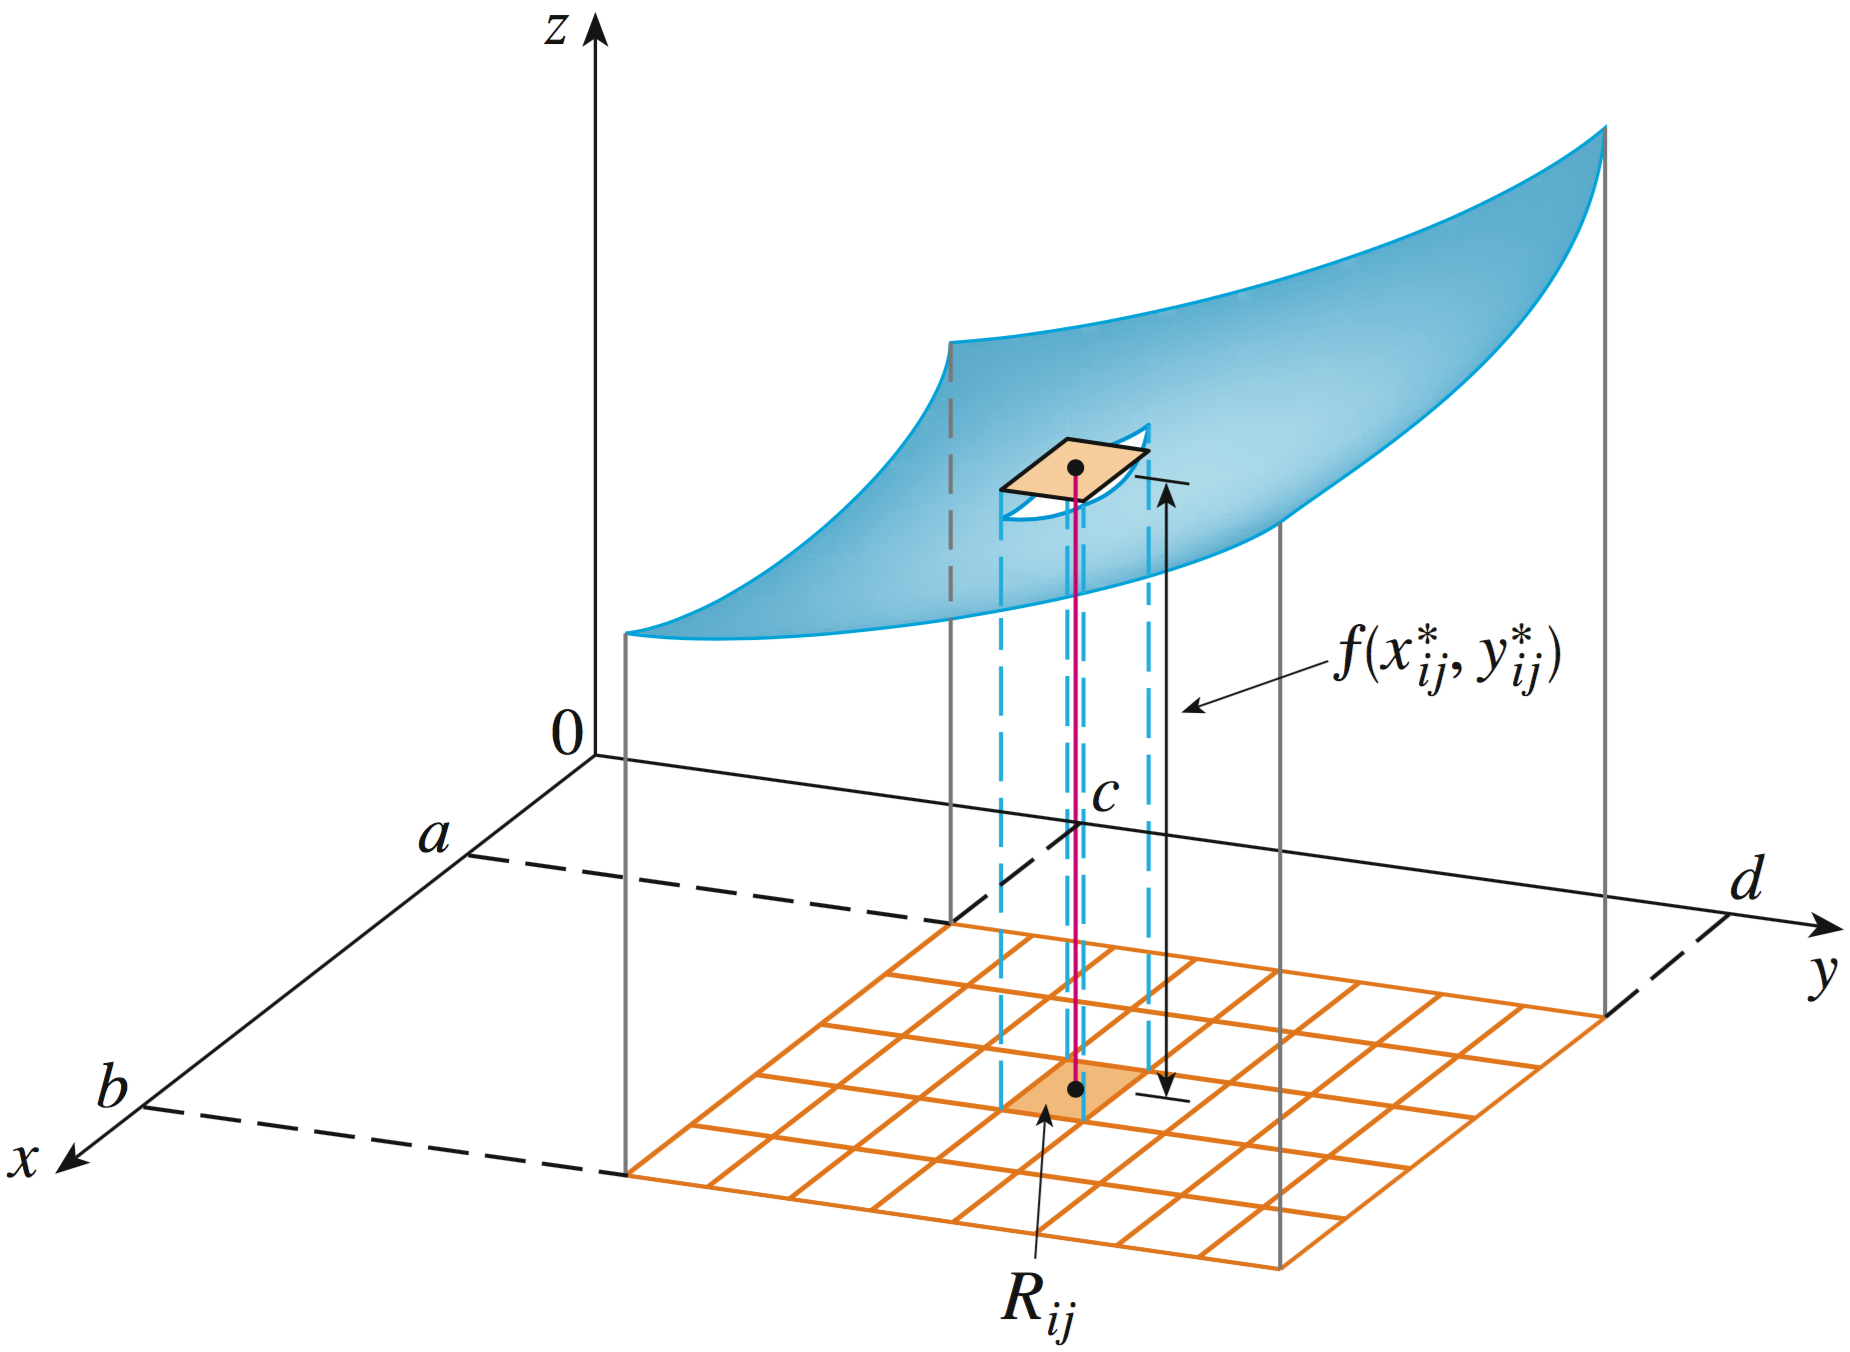
\includegraphics[width=5cm]{doubleint.png}
        \end{align*}
        The \textbf{double integral} of $f$ over the rectangle $R$ is defined as a double Riemann sum:
        \begin{align*}
            \iint_R f(x,y) \,dA = \lim_{m,n \rightarrow \infty} \sum_{i=1}^m \sum_{j=1}^n f(x_{ij}^*, y_{ij}^*) \Delta A
        \end{align*}
        If this limit exists, then $f$ is \textit{integrable}. Note that all continuous functions are integrable.
        % \item Methods for approximating single integrals (midpoint rule, trapezoidal rule, etc.) all have counterparts for double integrals. For example, the midpoint rule for double integrals involves choosing the sample point to be the center $(\bar{x_i}, \bar{y_i})$ of $R_{ij}$.
        % \item If $f(x,y) \geq 0$, the \textbf{volume} $V$ of the solid that lies above the rectangle $R$ and below the surface $f(x,y)$ is
        % $$ V = \iint_R f(x,y) \,dA $$
        \item It is of course impractical to compute double integrals from the definition, so we decompose double integrals into \textbf{iterated integrals}. Suppose $f(x,y)$ is integrable on $R=[a,b] \times [c,d]$. Then the notation 
        \begin{align*}
            \int_a^b \hspace{-1.8mm}\int_c^d f(x,y) \,dy \,dx 
        \end{align*}
        means perform partial integration with respect to $y$ from $y=c$ to $y=d$, then integrate the result with respect to $x$ from $x=a$ to $x=b$.
        \item Fubini's theorem: If $f$ is continuous on the closed rectangle $R= [a,b] \times [c,d]$, then
        \begin{align*}
            \iint_R f(x,y) \,dA &= \int_a^b \hspace{-1.8mm} \int_c^d f(x,y) \,dy \,dx \\ &= \int_c^d \hspace{-1.8mm} \int_a^b f(x,y) \,dx \,dy
        \end{align*}
        Hence it is wise to choose the order of integration that results in the simplest integrands.
        \item If $f(x,y)$ can be factored into a function of $x$ and a function of $y$ only, that is, $f(x,y) = g(x)h(y)$, then the double integral can be written as the product of single integrals:
        \begin{align*}
            \iint_R g(x)h(y) \,dA = \int_a^b g(x) \,dx \int_c^d h(y) \,dy
        \end{align*}
        This important result holds for triple integrals too.
        \item The \textbf{average value} of $f(x,y)$ defined on a rectangle $R$ is 
        \begin{align*}
            f_{avg} = \frac{1}{A_R} \iint_R f(x,y) \,dA
        \end{align*}
        where $A_R$ is the area of $R$.
    \end{enumerate}
    \item \textbf{Double Integrals over General Regions}
    \begin{enumerate} 
        \item Now we consider the case when we wish to integrate not just over rectangles but regions $D$ of a more general shape. 
        \item A plane region $D$ is said to be \textbf{type 1} if it lies between the curves of two continuous functions of $x$, that is,
        \begin{align*}
            D = \{(x,y) \mid a \leq x \leq b, g_1(x) \leq y \leq g_2(x) \}
        \end{align*}
        \vspace{-7mm}
        \begin{align*}
            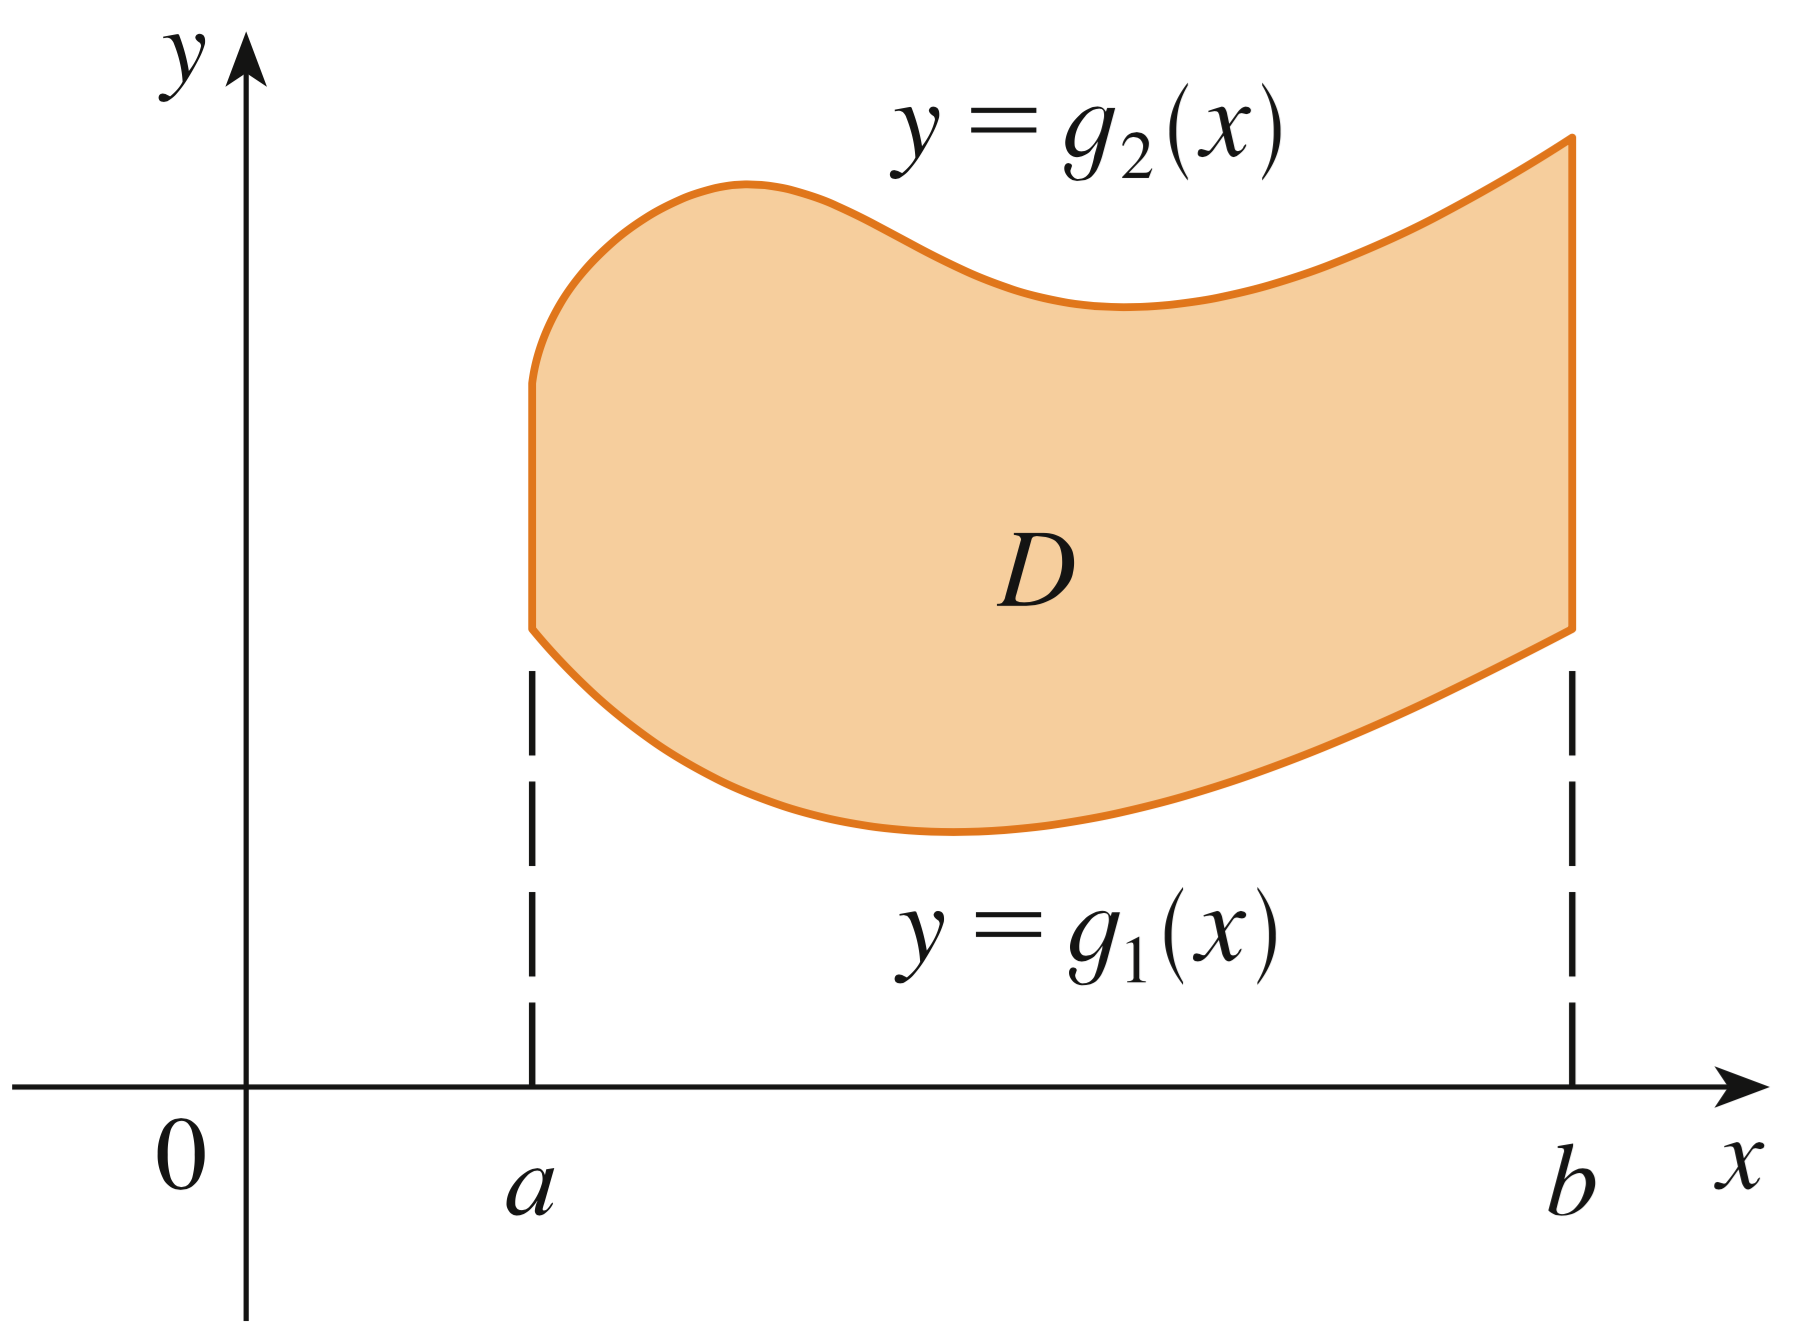
\includegraphics[width=4.3cm]{type1.png}
        \end{align*}
        If $f$ is continuous on a type 1 region $D$, then
        \begin{align*}
            \iint_D f(x,y) \,dA = \int_a^b \hspace{-1.5mm} \int_{g_1(x)}^{g_2(x)} f(x,y) \,dy \,dx
        \end{align*}
        \item A plane region $D$ is said to be \textbf{type 2} if it lies between the curves of two continuous functions of $y$, that is,
        \begin{align*}
            D = \{(x,y) \mid c \leq y \leq d, h_1(y) \leq x \leq h_2(y) \}
        \end{align*}
        \vspace{-7mm}
        \begin{align*}
            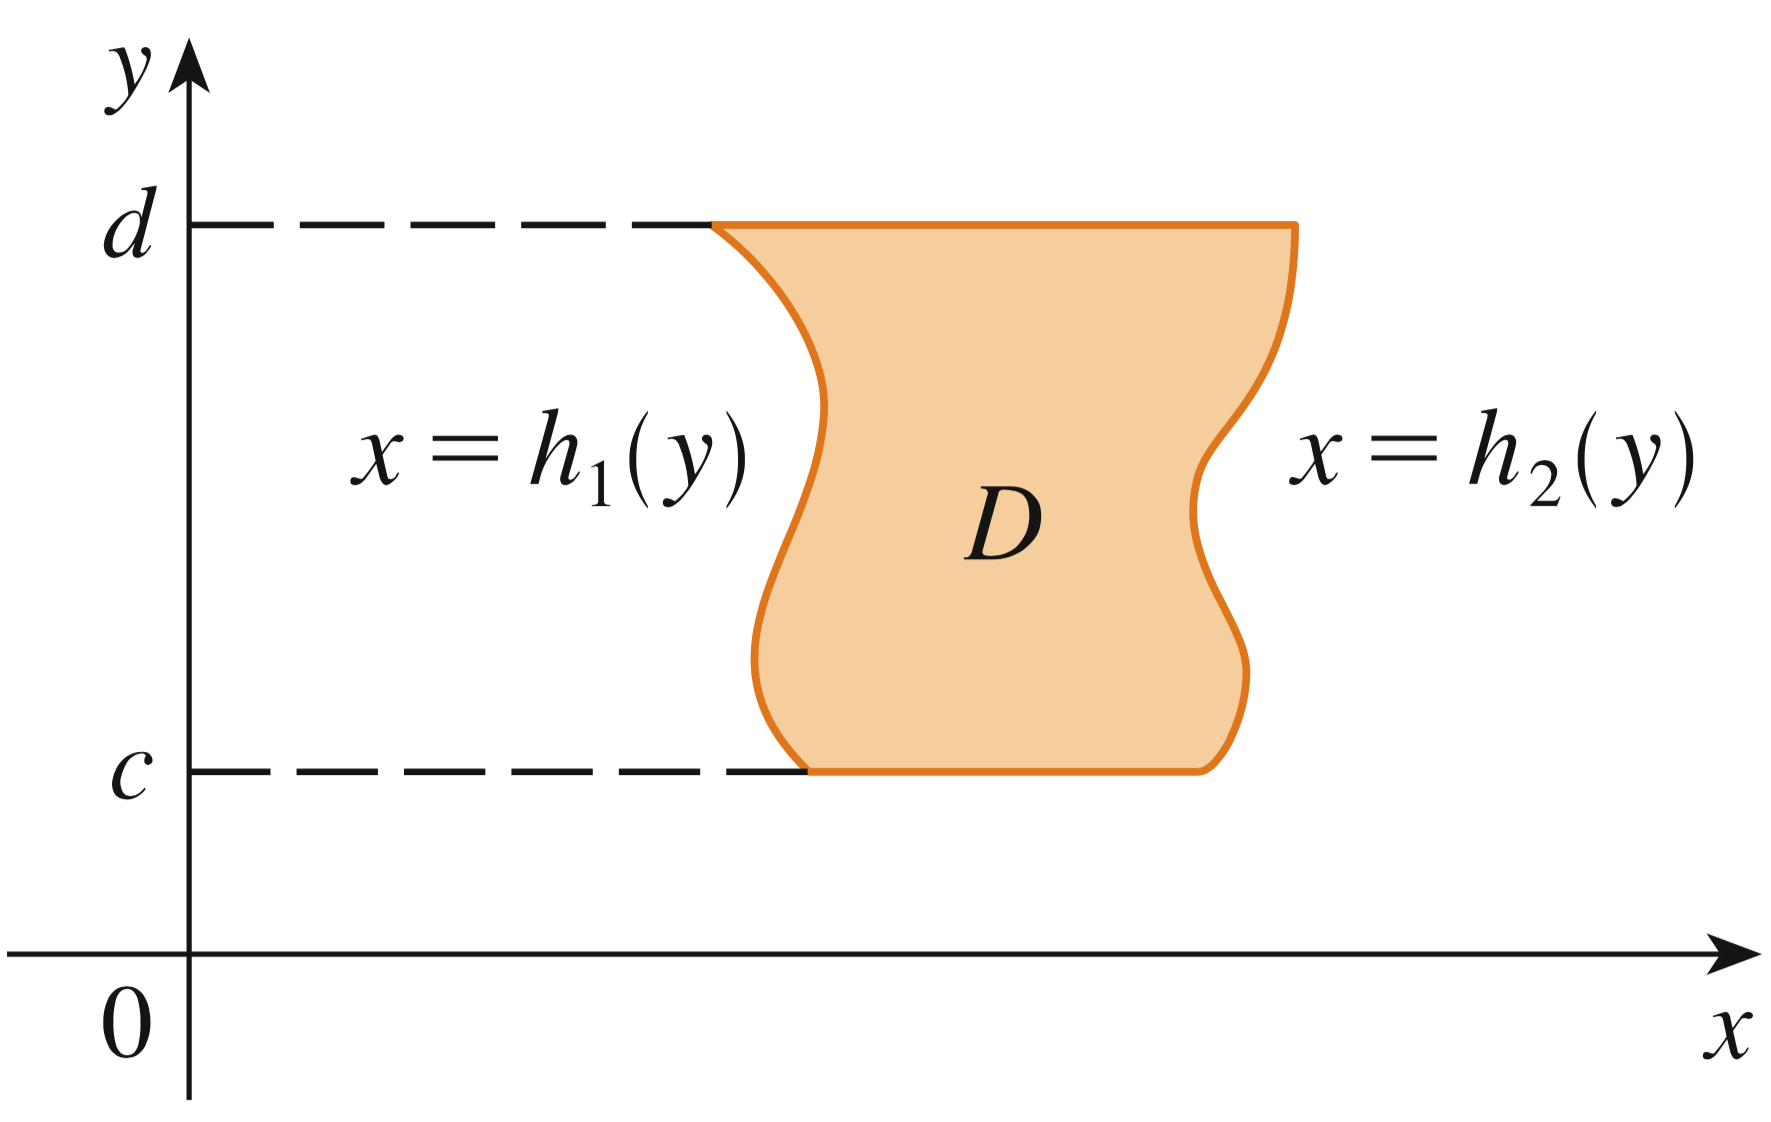
\includegraphics[width=4.7cm]{type2.png}
        \end{align*}
        If $f$ is continuous on a type 2 region $D$, then
        \begin{align*}
            \iint_D f(x,y) \,dA = \int_c^d \hspace{-1.5mm} \int_{h_1(y)}^{h_2(y)} f(x,y) \,dx \,dy
        \end{align*}
        \item A region can both type 1 and type 2, so choose the simpler description. A region can also be neither type 1 nor type 2; in such a case, try to decompose the region into a union of type 1 and type 2 regions.
        \item Changing the order of integration now requires extracting the region $D$ and providing an alternate description of it in terms of the other variable.
        \item Properties of Double Integrals:
        \begin{itemize}
            \item $\iint_D [f(x,y) + g(x,y)] \,dA = \iint_D f(x,y) \,dA + \iint_D g(x,y) \,dA$
            \item $\iint_D cf(x,y) \,dA = c \iint_D f(x,y) \,dA$
            \item If $\alpha \leq f(x,y) \leq \beta$ for all $(x,y) \in D$, then $\alpha A_D \leq \iint_D f(x,y) \,dA \leq \beta A_D$
        \end{itemize} 
        
        \item Calculating the double integral of the constant $1$ over a region $D$ yields the area of $D$.
        
    \end{enumerate}
    
    \item \textbf{Double Integrals in Polar Coordinates}
    \begin{enumerate}
        \item Sometimes a region can be more easily described using polar coordinates. Consider a general polar region $D$:
        \begin{align*}
            D = \{(r, \theta) \mid \alpha \leq \theta \leq \beta, h_1(\theta) \leq r \leq h_2(\theta) \}
        \end{align*}
        \vspace{-7mm}
        \begin{align*}
            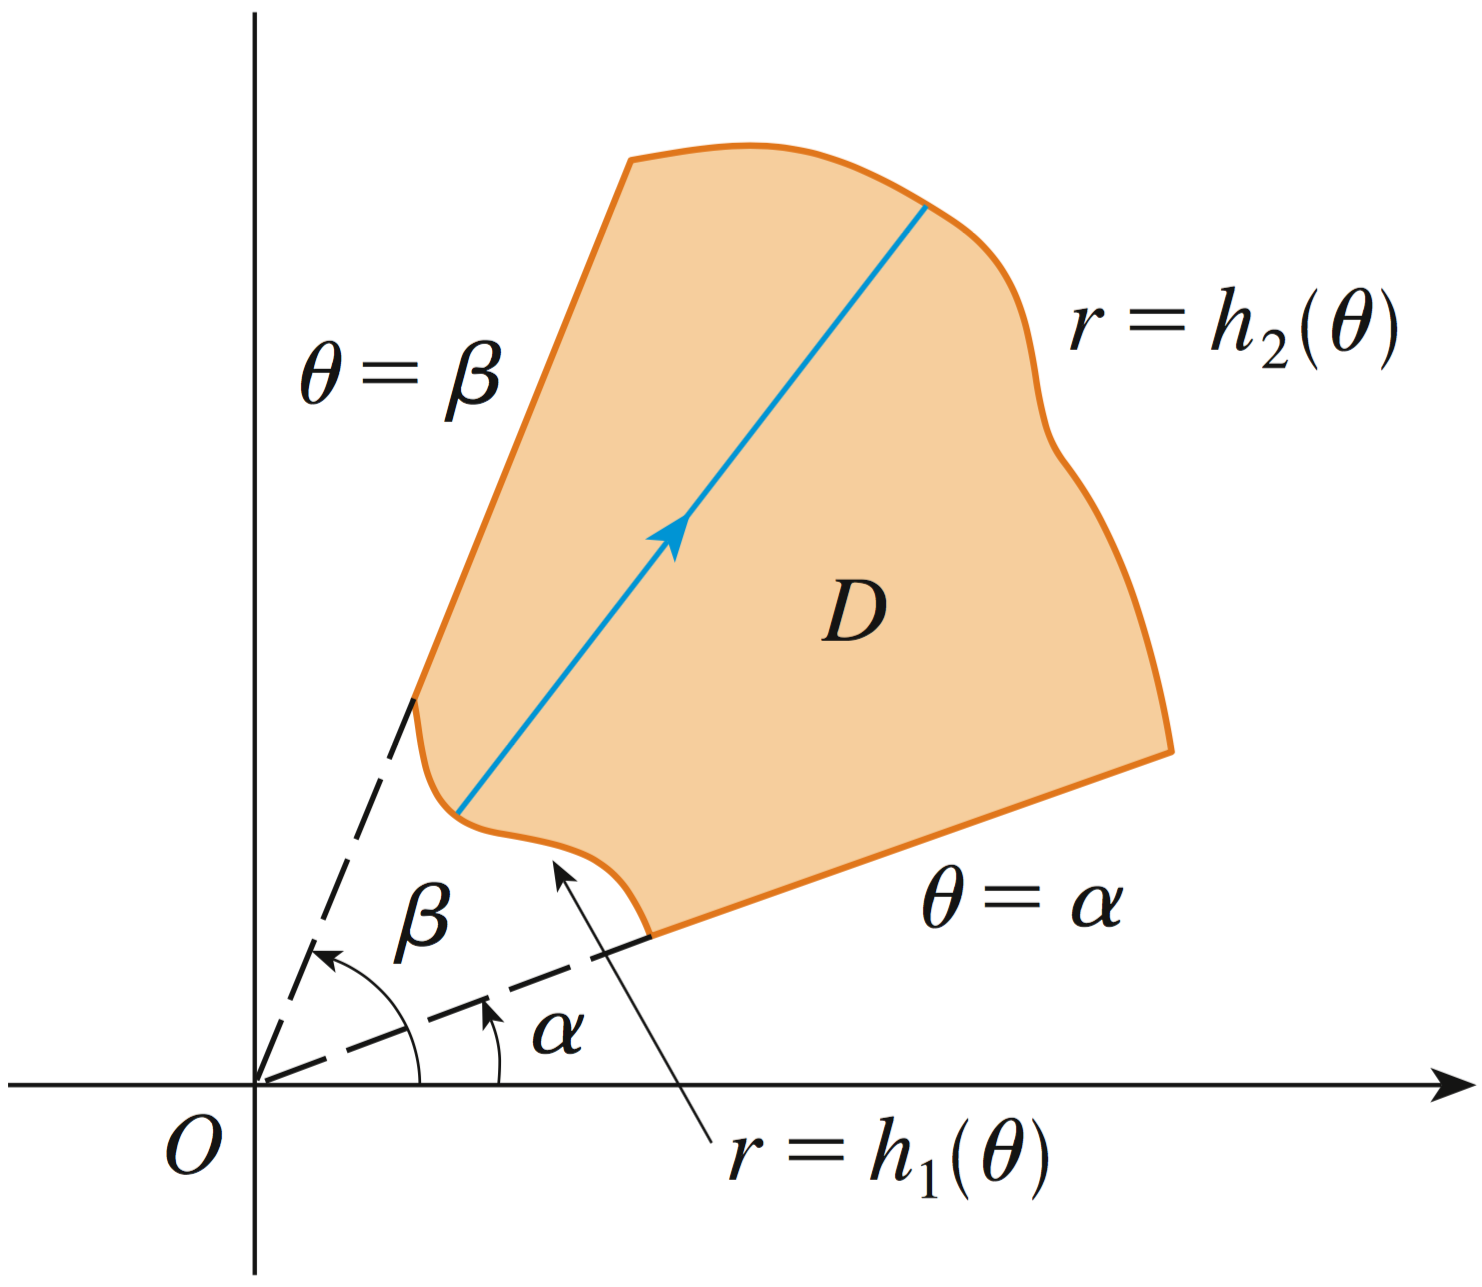
\includegraphics[width=4cm]{polar.png}
        \end{align*}
        If $f$ is continuous on a polar region $D$, then
        \begin{align*}
            \iint_D f(x,y) \,dA = \int_\alpha^\beta \hspace{-1.5mm} \int_{h_1(\theta)}^{h_2(\theta)} f(r\cos{\theta}, r\sin{\theta})r \,dr \,d\theta
        \end{align*}
        \item Convert a double integral in Cartesian coordinates into a double integral in Polar coordinates by taking $x = r \cos{\theta}$, $y=r\sin{\theta}$ and determining the appropriate limits of integration. 
    \end{enumerate}
    \item \textbf{Applications of Double Integrals}
    \begin{enumerate}
        \item \textbf{Density and Mass} \\ A \textbf{lamina} is a two-dimensional planar closed surface with mass and density. Let $\mathcal{L}$ be a lamina of uniform density bounded by the curves $y=f(x)$, $y=g(x)$, $x=a$, and $x=b$, where $f(x) \geq g(x)$ and $b \geq a$. The \textbf{centroid}, or center of mass, of $\mathcal{L}$ is $(\bar{x}, \bar{y})$, where 
        \begin{align*}
            \bar{x} &= \frac{1}{A} \int_a^b x[f(x) - g(x)] \,dx \\
            \bar{y} &= \frac{1}{A} \int_a^b \frac{1}{2} [f(x)^2 - g(x)^2] \,dx\textbf{}
        \end{align*}
        and $A$ is the area of the lamina, i.e. $A=\int_a^b [f(x) - g(x)] \,dx$. 
    \item Now we consider a lamina of variable density. Suppose a lamina occupies a region $D$ in the plane and its density (mass per unit area) at a point $(x,y)$ is given by $\rho(x,y)$, where $\rho$ is a continuous function on $D$. Then the \textbf{total mass $m$ of the lamina} is 
    \begin{align*}
        m = \iint_D \rho(x,y) \,dA
    \end{align*}
   The \textbf{center of mass} of the lamina is $(\bar{x}, \bar{y})$, where
   \begin{align*}
       \bar{x} = \frac{M_y}{m} = \frac{1}{m} \iint_D x \rho(x,y) \,dA \\
       \bar{y} = \frac{M_x}{m} = \frac{1}{m} \iint_D y \rho(x,y) \,dA 
   \end{align*}
   The quantities $M_x$ and $M_y$ are called the moment about the $x$-axis and moment about the $y$-axis, respectively.
   \item \textbf{Continuous Probability} \\ Recall the \textbf{probability density function} (PDF) of a continuous random variable $X$ is a real-valued function $f(x)$ such that $f(x) \geq 0$ and $\int_{\mathbb{R}} f(x) \,dx=1$. We define the probability that $X$ lies in some interval $[a,b]$ as $$P(X \in [a,b]) = \int_a^b f(x) \,dx$$
   \item Also recall a random variable $X$ is \textit{exponentially distributed} if its PDF is of the form $$f(x) = \lambda e^{-\lambda x}$$ so that $E(X) = \frac{1}{\lambda}$ and Var($X)=\frac{1}{\lambda^2}$. A random variable $X$ is \textit{normally distributed} if its PDF is of the form $$f(x) = \frac{1}{\sqrt{2\pi\sigma^2}}e^{-(x-\mu)^2 / 2\sigma^2}$$ so that $E(X)=\mu$ and Var($X)=\sigma^2$.
   \item Now we consider two continuous random variables $X$ and $Y$. The \textbf{joint density function} of $X$ and $Y$ is a function $f(x,y)$ such that $f(x,y) \geq 0$ and $\iint_{\mathbb{R}^2} f(x,y) \,dA = 1$. We define the probability that $X$ and $Y$ lie in a region $D$ as 
   $$P((X,Y) \in D) = \iint_D f(x,y) \,dA$$
   If $X$ and $Y$ are random variables with PDFs $f_X$ and $f_Y$, respectively, then $X$ and $Y$ are \textbf{independent} iff their joint density function is a product of their individual PDFs: $$f(x,y) = f_X(x) f_Y(y)$$
   \item If $X$ and $Y$ are random variables with joint density function $f$, define the expected values of $X$ and $Y$ to be
   \begin{align*}
       E(X) = \iint_{\mathbb{R}^2} x f(x,y) \,dA \\
       E(Y) = \iint_{\mathbb{R}^2} y f(x,y) \,dA 
   \end{align*}
    
    \end{enumerate}
    
    \columnbreak
    \item \textbf{Triple Integrals}
    \begin{enumerate}
        \item Analogous to double integrals, we define triple integrals for functions of three variables as a triple Riemann sum over a box.
        \item If $f(x,y,z)$ is continuous on the box $B=[a,b] \times [c,d] \times [r,s]$, then
        \begin{align*}
            \iiint_B f(x,y,z) \,dV = \int_r^s \hspace{-1.8mm} \int_c^d \hspace{-1.8mm} \int_a^b f(x,y,z) \,dx \,dy \,dz
        \end{align*}
        By Fubini's theorem, there are six possible orderings that yield the same result.
        \item As before, now we consider triple integrals over a general bounded region $E$, which is now a solid.
        \item A solid region $E$ is said to be \textbf{type 1} if it lies between the graphs of two continuous functions of $x$ and $y$, that is, \begin{align*}
            E = \{ (x,y,z) \mid (x,y) \in D, u_1(x,y) \leq z \leq u_2(x,y) \}
        \end{align*}
        where $D$ is the projection of $E$ onto the $xy$-plane.
        \vspace{-4mm}
        \begin{align*}
            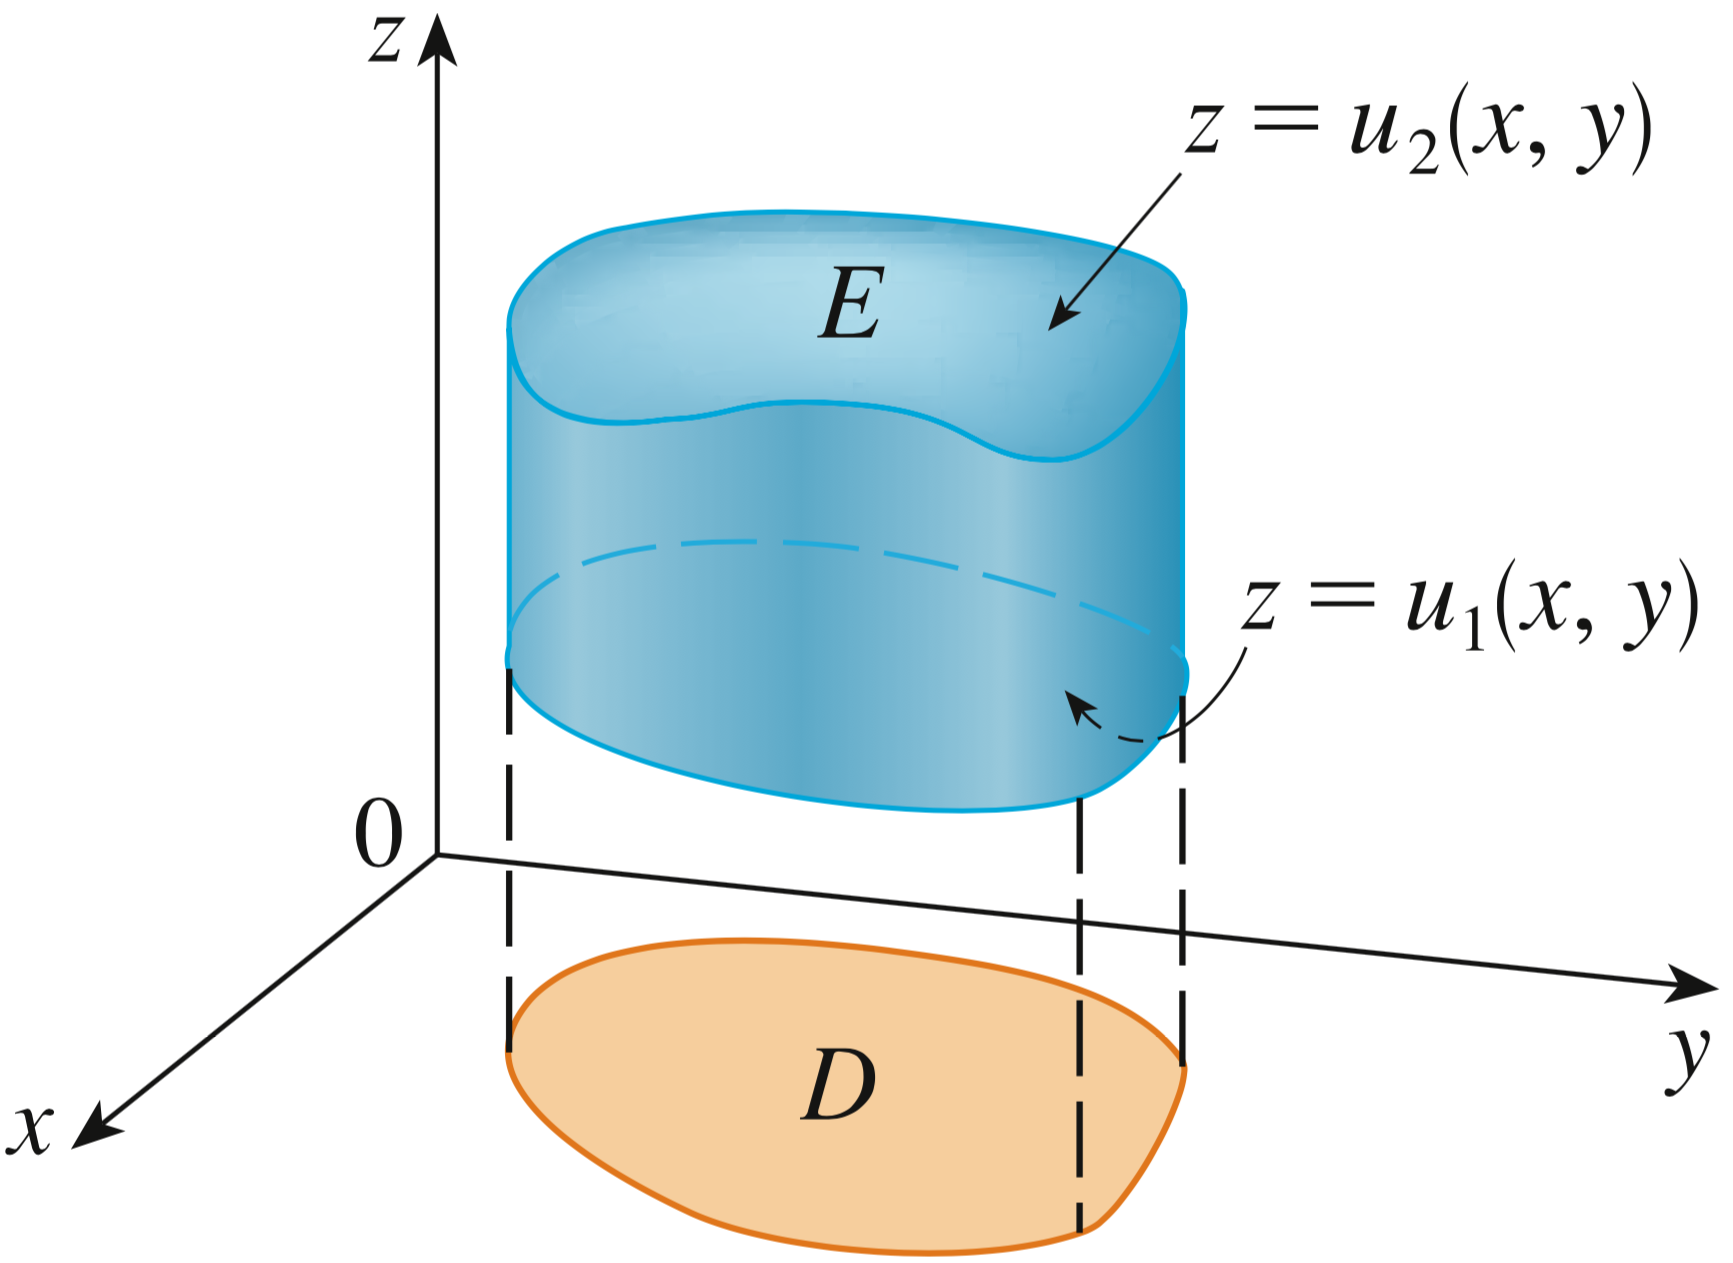
\includegraphics[width=4.1cm]{type1t.png}
        \end{align*}
        In this case, we have
        \begin{align*}
            \iiint_E f(x,y,z) \,dV = \iint_D \left[ \int_{u_1(x,y)}^{u_2(x,y)} f(x,y,z) \,dz \right] \,dA
        \end{align*}
        \item Similarly, a \textbf{type 2} solid region $E$ is of the form
        \begin{align*}
            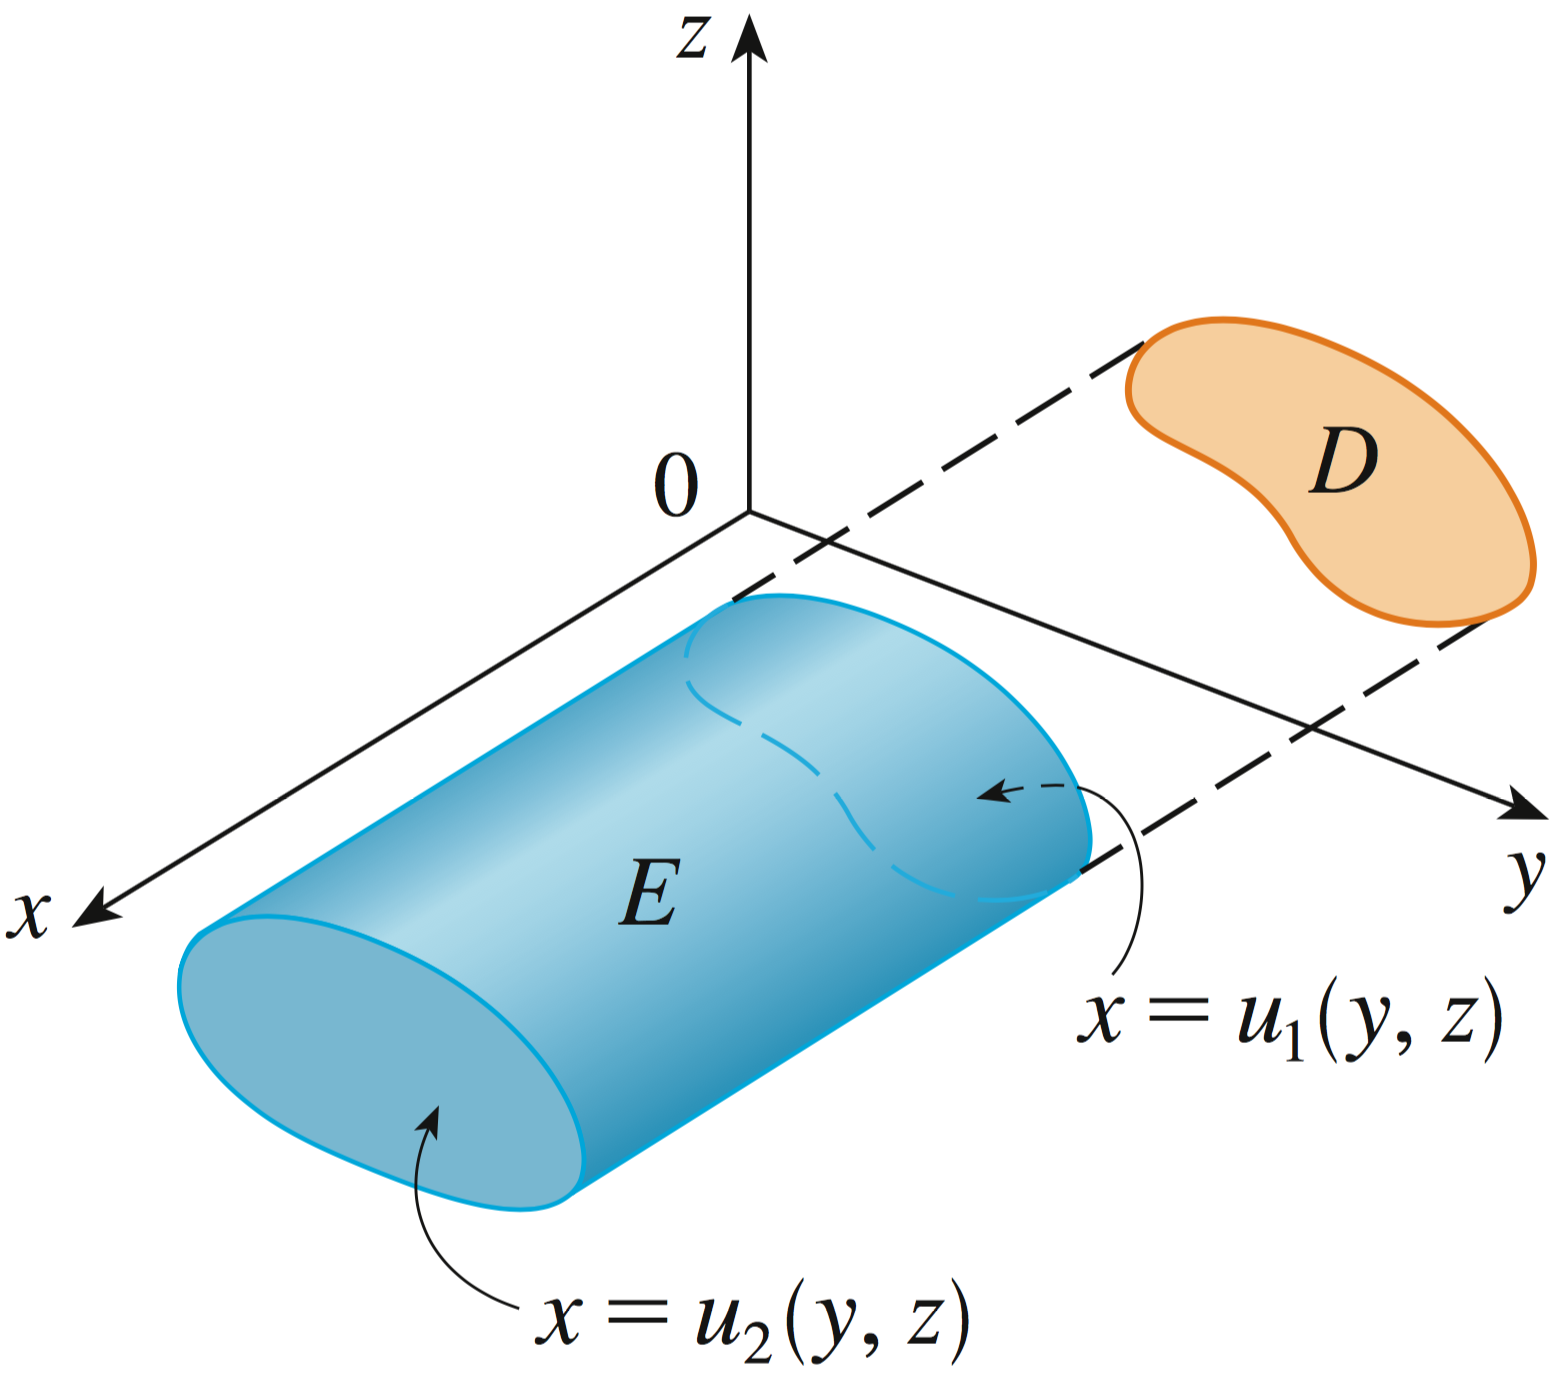
\includegraphics[width=4cm]{type2t.png}
        \end{align*}
        We have
        \begin{align*}
            \iiint_E f(x,y,z) \,dV = \iint_D \left[ \int_{u_1(y,z)}^{u_2(y,z)} f(x,y,z) \,dx \right] \,dA
        \end{align*}
        \item Lastly, a \textbf{type 3} solid region $E$ is of the form
        \begin{align*}
            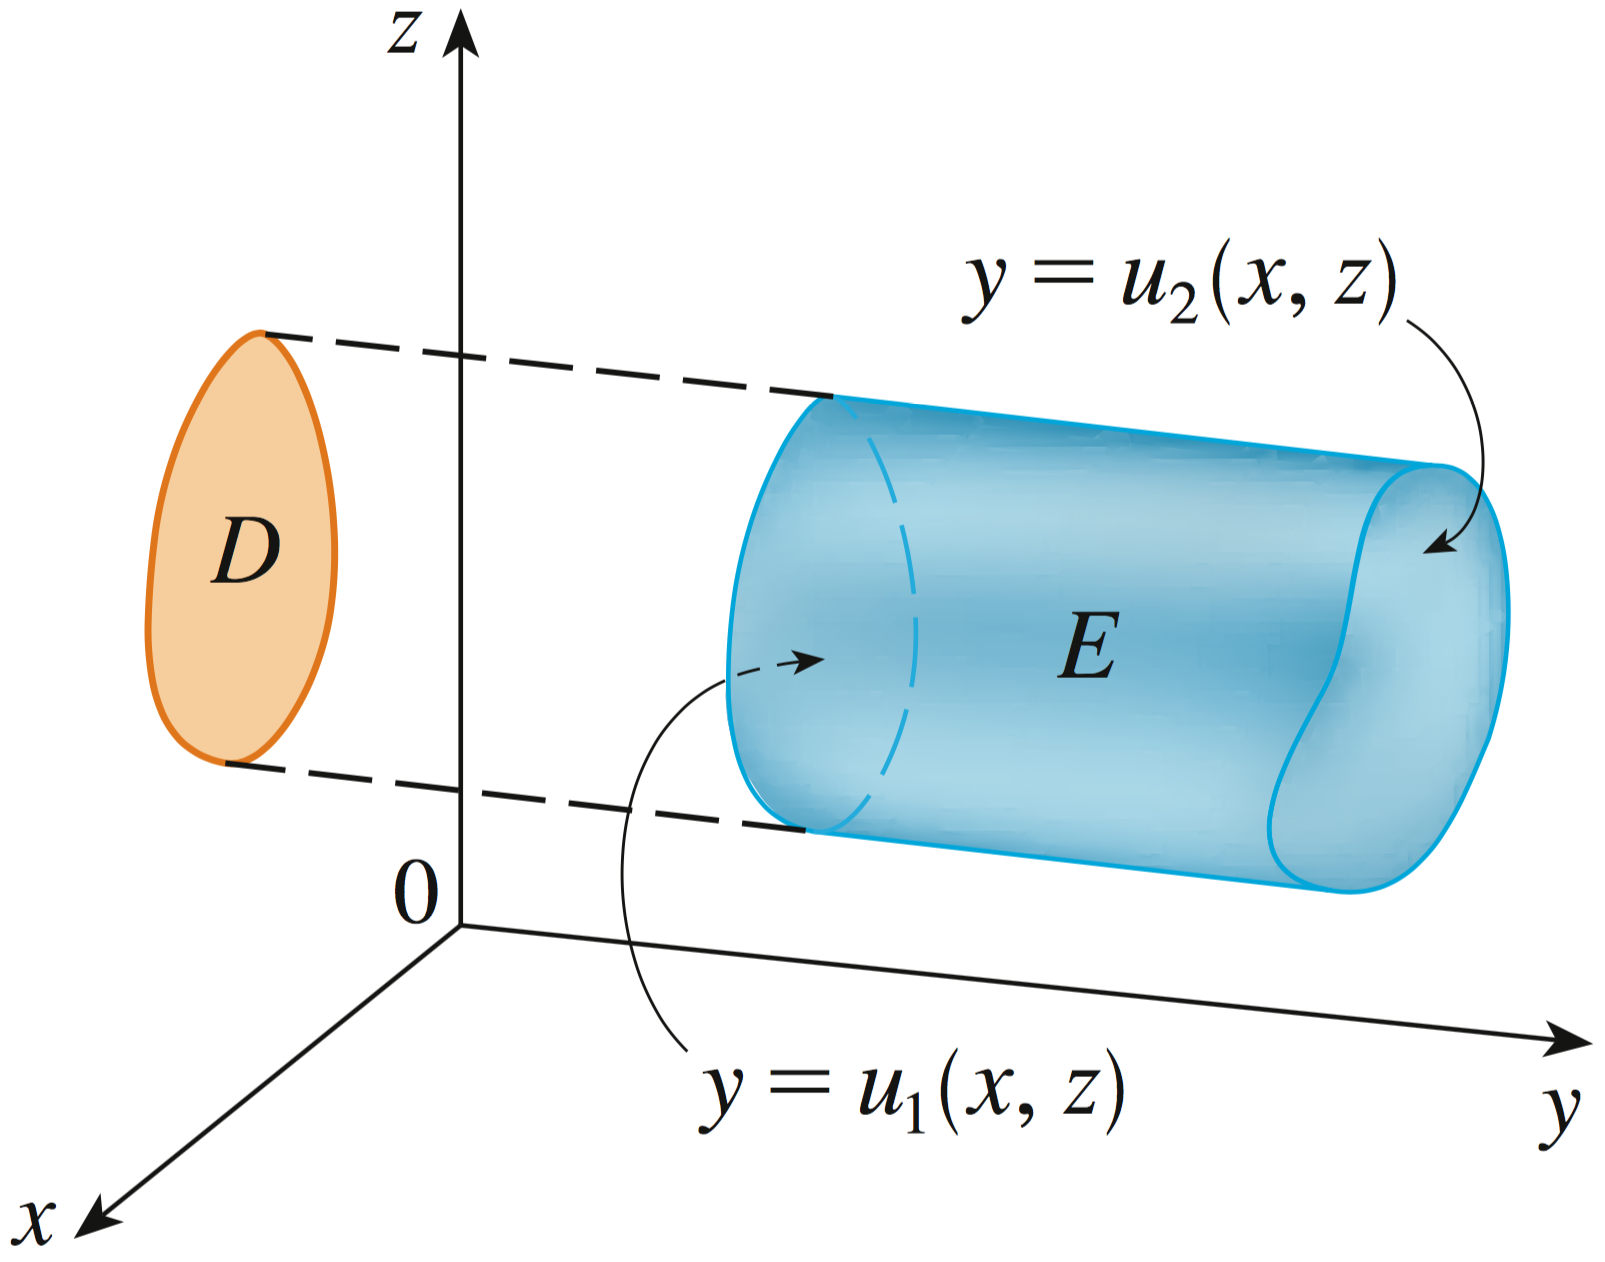
\includegraphics[width=4cm]{type3t.png}
        \end{align*}
        We have
        \begin{align*}
            \iiint_E f(x,y,z) \,dV = \iint_D \left[ \int_{u_1(x,z)}^{u_2(x,z)} f(x,y,z) \,dy \right] \,dA
        \end{align*}
        \item Each of these three cases involves a double integral. In order to evaluate the outer double integral, we must classify the projection $D$ as a type 1 plane region or type 2 plane region, and then proceed as before. It is wise to draw a diagram of the solid $E$ as well as its projection $D$ in computing triple integrals.
        \item The corresponding interpretation of a triple integral is the hypervolume of a four-dimensional object, which is not very useful. However, calculating the triple integral of the constant $1$ over a region $E$ yields the volume of $E$.
        \item Suppose a solid object occupies a region $E$ and its density (mass per unit volume) at a point $(x,y,z)$ is given by $\rho(x,y,z)$. The total mass $m$ of the solid is
        \begin{align*}
            m = \iiint_E \rho(x,y,z) \,dV
        \end{align*}
        Its moments about the three coordinate planes are
        \begin{align*}
            M_{yz} = \iiint_E x\rho(x,y,z) \,dV \\
            M_{xz} = \iiint_E y\rho(x,y,z) \,dV \\
            M_{xy} = \iiint_E z\rho(x,y,z) \,dV
        \end{align*}
        The center of mass is located at $(\bar{x},\bar{y},\bar{z})$, where 
        \begin{align*}
            \bar{x} = \frac{M_{yz}}{m} \hspace{7mm} \bar{y} = \frac{M_{xz}}{m} \hspace{7mm} \bar{z} = \frac{M_{xy}}{m}
        \end{align*}
        If the density is constant, the center of mass is called the centroid of $E$.
    \end{enumerate}
    \item \textbf{Triple Integrals in Cylindrical Coordinates}
    \begin{enumerate}
        \item In the \textbf{cylindrical coordinate system}, a point $P$ in three-dimensional space is represented by the ordered triple $(r, \theta, z)$ where $r$ and $\theta$ are polar coordinates of the projection of $P$ onto the $xy$-plane and $z$ is the directed distance from the $xy$-plane to $P$.
        \item The relationship between rectangular and cylindrical coordinates is given by
            $$x = r\cos{\theta} \hspace{7mm} y = r\sin{\theta} \hspace{7mm} z= z$$
            $$r^2=x^2+y^2 \hspace{7mm} \tan{\theta} = \frac{y}{z} \hspace{7mm} z=z$$
        \item Suppose $E$ is a type 1 region whose projection $D$ onto the $xy$-plane is conveniently described in polar coordinates. 
        \begin{align*}
            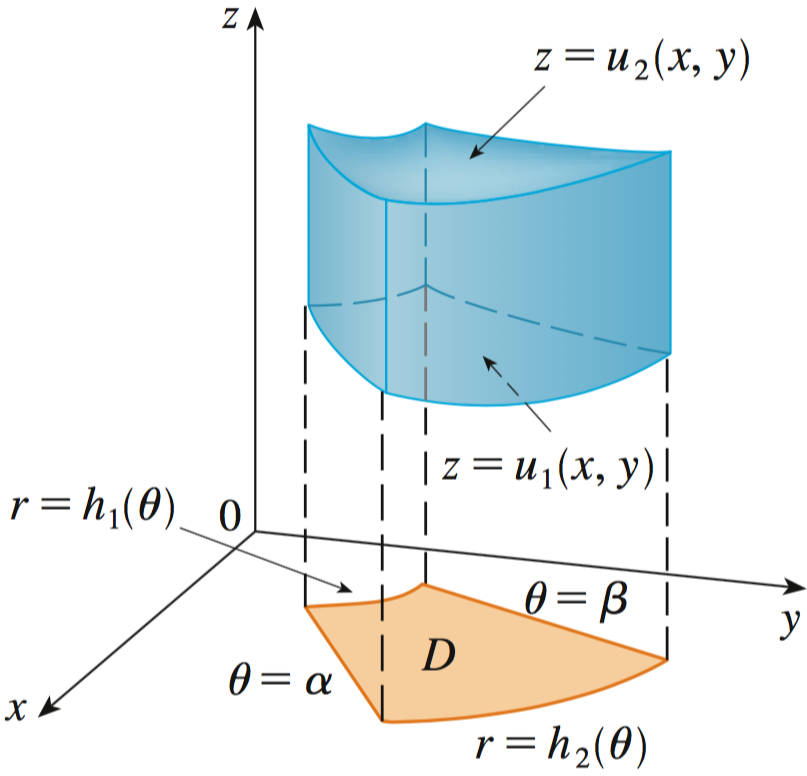
\includegraphics[width=4.2cm]{cyl.png}
        \end{align*}
        Combining results from earlier, we have
        \begin{align*}
        \hspace{-5mm}
            &\iiint_E f(x,y,z) \,dV = \\
        \hspace{-5mm}
            &\int_\alpha^\beta \hspace{-1.8mm} \int_{h_1(\theta)}^{h_2(\theta)} \hspace{-1.8mm} \int_{u_1(r\cos{\theta}, r\sin{\theta})}^{u_2(r\cos{\theta}, r\sin{\theta})} f(r\cos{\theta}, r\sin{\theta},z) r \,dz \,dr \,d\theta
        \end{align*}
        \item It is worthwhile to convert a triple integral from rectangular to cylindrical coordinates if $E$ is a solid region easily described in cylindrical coordinates (e.g., symmetrical about $z$-axis), and especially when $f(x,y,z)$ involves the expression $x^2+y^2$.
    \end{enumerate}
    \item \textbf{Triple Integrals in Spherical Coordinates}
    \begin{enumerate}
        \item In the \textbf{spherical coordinate system}, a point $P$ in three-dimensional space is represented by $(\rho, \theta, \phi)$, where $\rho$ is the distance from $P$ to the origin $O$, $\theta$ is the same as in cylindrical coordinates, and $\phi$ is the angle between the positive $z$-axis and line segment $OP$. Note that $\rho \geq 0$ and $0 \leq \phi \leq \pi$.
        \begin{align*}
            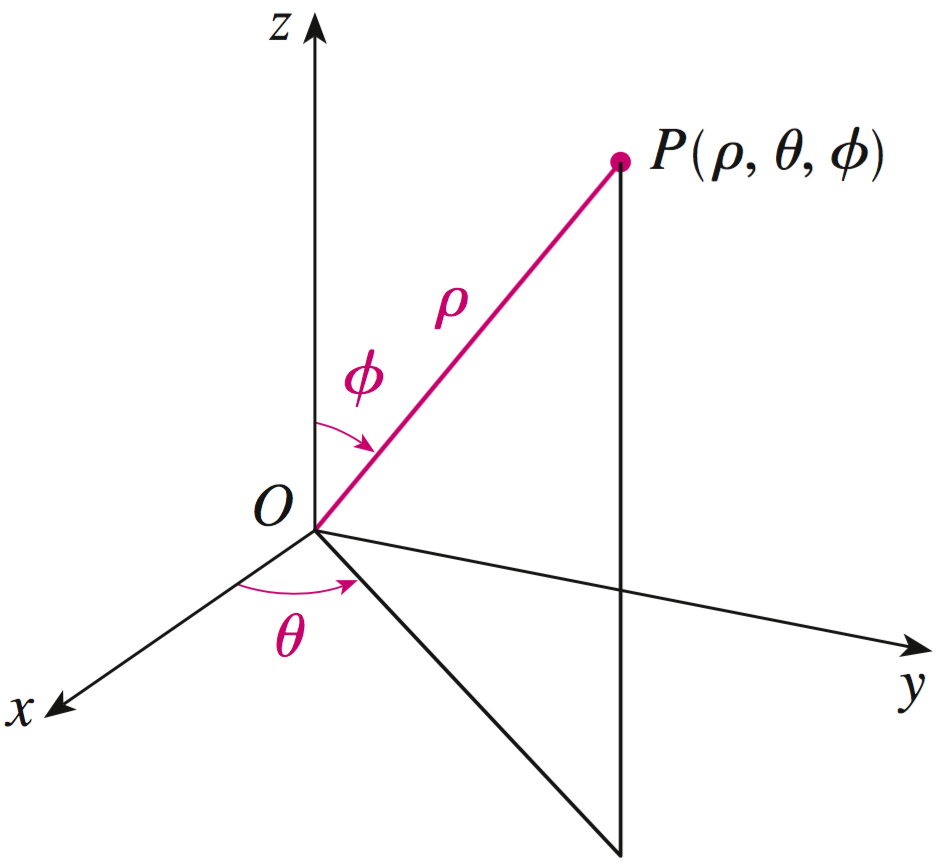
\includegraphics[width=3.5cm]{spher.png}
        \end{align*}
        \item The relationship between rectangular and spherical coordinates is given by
            $$x = \rho \sin{\phi}\cos{\theta} \hspace{7mm} y = \rho \sin{\phi}\sin{\theta} \hspace{7mm} z = \rho\cos{\phi}$$
            $$\rho^2 = x^2 + y^2 + z^2$$
        \item We have
        \begin{align*}
        \hspace{-5mm}
            &\iiint_E f(x,y,z) \,dV = \\
        \hspace{-5mm}
            &\int_c^d \hspace{-1.8mm} \int_\alpha^\beta \hspace{-1.8mm} \int_{a}^{b} \hspace{-1.8mm} f(\rho\sin{\phi}\cos{\theta}, \rho \sin{\phi}\sin{\theta}, \rho\cos{\phi}) \rho^2 \sin{\phi} \,d\rho \,d\theta \,d\phi
        \end{align*}
        where $E$ is a spherical wedge given by 
        \begin{align*}
            E = \{ (\rho, \theta, \phi) \mid a \leq \rho \leq b, \alpha \leq \theta \leq \beta, c \leq \phi \leq d \}
        \end{align*}
        % \item We can extend this to more general spherical regions by replacing the limits of integration for $\rho$ with $g_1(\theta, \phi)$ and $g_2(\theta, \phi)$.
        % \item Spherical coordinates can be convenient in triple integrals when surfaces such as cones and spheres form the boundary of the region of integration.
    \end{enumerate}
    
    \item \textbf{Change of Variables in Multiple Integrals}
    \begin{enumerate}
        \item In single-variable calculus we often used a change of variable (or $u$-substitution) to simplify an integral. 
        \item Now we consider more generally a change of variables given by a transformation $T$ from the $uv$-plane to the $xy$-plane, where $x$ and $y$ are related to $u$ and $v$ by
        \begin{align*}
            x = g(u,v) \hspace{8mm} y = h(u,v)
        \end{align*}
        The goal is generally to transform a region $R$ in $xy$-coordinates into a region in $uv$-coordinates that is easier to describe.
        \item The \textbf{Jacobian} of the transformation $T$ given by $x=g(u,v)$ and $y=h(u,v)$ is the determinant
        \begin{align*}
            \frac{\partial (x,y)}{\partial (u,v)}  =
            \begin{vmatrix}
                \frac{\partial x}{\partial u} & \frac{\partial x}{\partial v} \\[8pt]
                \frac{\partial y}{\partial u} & \frac{\partial y}{\partial v}
            \end{vmatrix}
        \end{align*}
        \item \textit{Change of variables in a double integral}: Let $T$ be a one-to-one transformation whose Jacobian is nonzero that maps a region $S$ in the $uv$-plane to a region $R$ in the $xy$-plane. Let $f$ be a continuous function on $R$, and that $R$ and $S$ are type 1 or type 2 plane regions. Then
        \begin{align*}
            \iint_R f(x,y) \,dA = \iint_S f(g, h) \left| \frac{\partial (x,y)}{\partial (u,v)} \right| \,du \,dv
        \end{align*}
        \item In other words, we convert an integral in $x$ and $y$ into an integral in $u$ and $v$ by expressing $x$ and $y$ in terms of $u$ and $v$ and writing $dA = \left| \frac{\partial (x,y)}{\partial (u,v)} \right| \,du \,dv$. Observe that in the single-variable case, the Jacobian is $\frac{dx}{du}$, which yields the familiar formula for $u$-substitution. 
        \item When the region of integration $R$ is too difficult to describe, construct a transformation $T$ from the $xy$-plane to a region $S$ in the $uv$-plane such that the images of the boundaries of $R$ under $T$ are simpler. Use $S$ to determine the new limits of integration and complete the change of variable to evaluate the integral.
        \item The formula for double integration in polar coordinates is just a special case of the above, which results from using the transformation $T$ from the $r\theta$-plane to the $xy$-plane given by $x=r\cos{\theta}$ and $y=r\sin{\theta}$.
        \item Now we consider triple integrals. Let $T$ be a transformation that maps a region $S$ in $uvw$-space onto a region $R$ in $xyz$-space by means of 
        \begin{align*}
            x=g(u,v,w) \hspace{7mm} y=h(u,v,w) \hspace{7mm} z=k(u,v,w)
        \end{align*}
        The Jacobian of $T$ is the $3 \times 3$ determinant
        \begin{align*}
            \frac{\partial (x,y,z)}{\partial (u,v,w)} = 
            \begin{vmatrix}
                \frac{\partial x}{\partial u} & \frac{\partial x}{\partial v} & \frac{\partial x}{\partial w} \\[8pt]
                \frac{\partial y}{\partial u} & \frac{\partial y}{\partial v} & \frac{\partial y}{\partial w} \\[8pt]
                \frac{\partial z}{\partial u} & \frac{\partial z}{\partial v} & \frac{\partial z}{\partial w} 
            \end{vmatrix}
        \end{align*}
        \item \textit{Change of variables in a triple integral}: Using similar hypotheses to those for double integrals, we have
        \begin{align*}
        \hspace{-5mm}
            &\iiint_R f(x,y,z) \,dV = \iiint_S f(g, h, k) \left| \frac{\partial (x,y,z)}{\partial (u,v,w)} \right| \,du \,dv \,dw
        \end{align*}
        where $g,h,k$ are the functions of $u,v,w$ defined earlier.
        \item The formulas for triple integration in cylindrical and spherical coordinates are just special cases of the above, using the appropriate relations. 
    \end{enumerate}
\end{enumerate}

\section{Vector Calculus}
\begin{enumerate}
    \item \textbf{Vector Fields}
    \begin{enumerate}
        \item Let $D$ be a subset of $\mathbb{R}^2$ and $E$ be a subset of $\mathbb{R}^3$. A \textbf{vector field} on $\mathbb{R}^2$ is a function $\vec{F}$ that assigns to each point $(x,y) \in D$ a vector $\vec{F}(x,y)$. Similarly, a vector field on $\mathbb{R}^3$ is a function $\vec{F}$ that assigns to each point $(x,y,z)\in E$ a vector $\vec{F}(x,y,z)$.
        \item $\vec{F}$ can be written in terms of its component functions $P, Q$ (or $P, Q, R$ in $\mathbb{R}^3$) as follows:
        \begin{align*}
            \vec{F}(x,y) = P(x,y)\vec{i} + Q(x,y)\vec{j} = \langle P(x,y), Q(x,y) \rangle
        \end{align*}
        \item A vector field on $D$ is usually visualized by drawing the vector $\vec{F}(x,y)$ starting at the point $(x,y)$ for a few representable points in $D$. \vspace{-2mm}
        \begin{align*}
            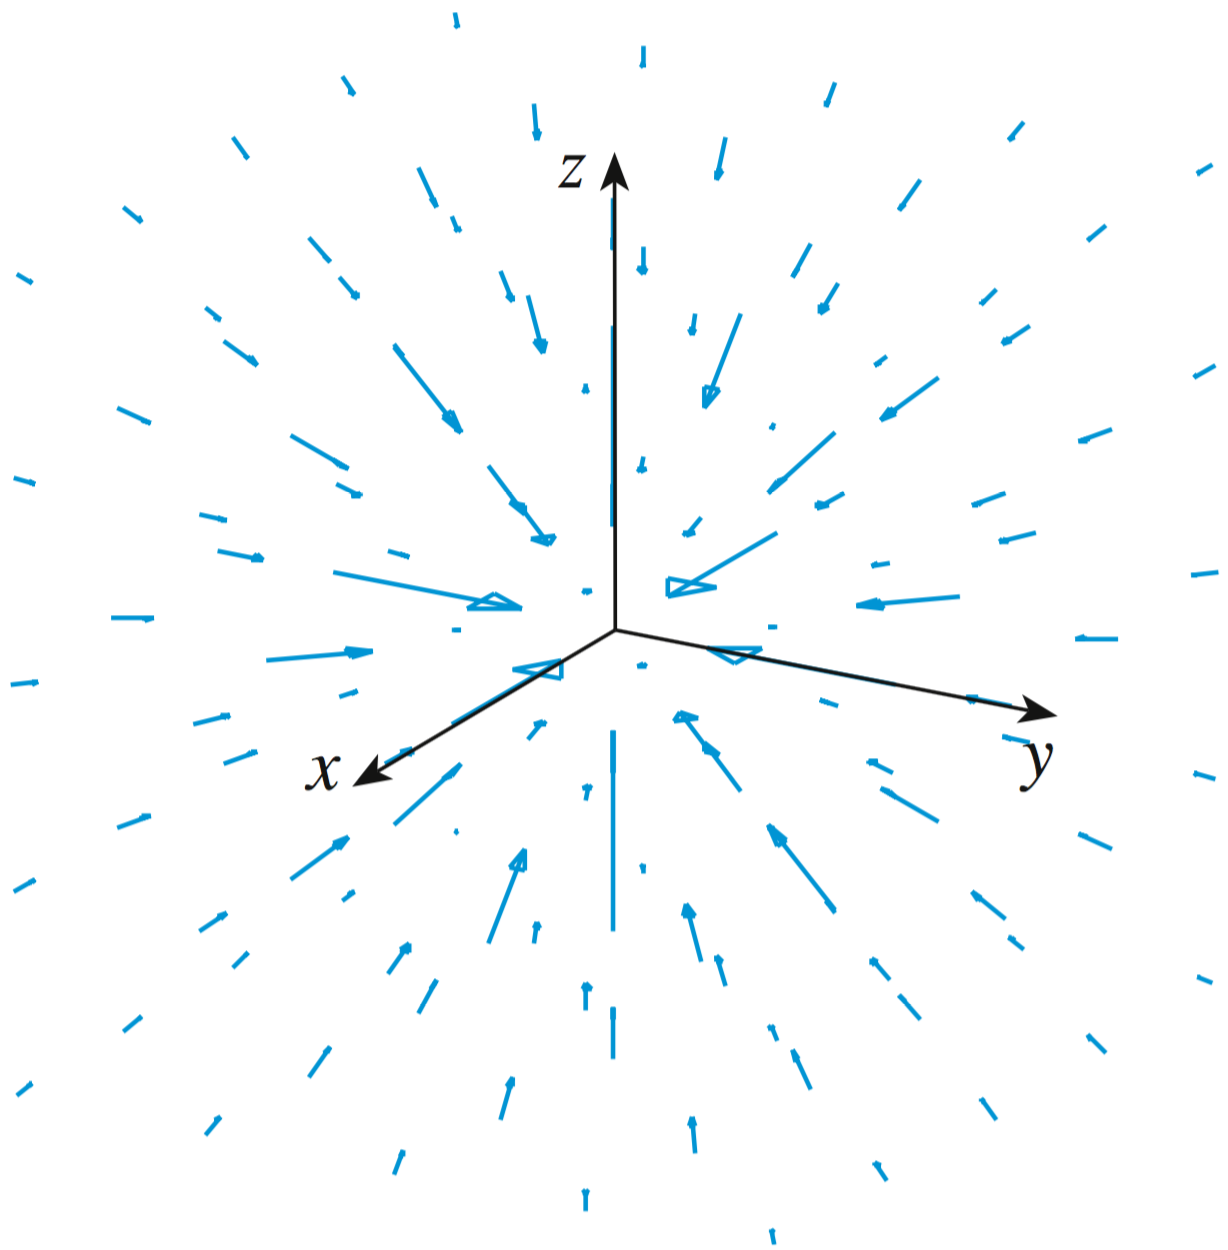
\includegraphics[width=3.2cm]{grav_field.png}
        \end{align*}
        \item A common vector field in physics is a \textbf{velocity field} $\vec{V}$, which assigns a velocity vector $\vec{V}(x,y,z)$ to each point $(x,y,z)$ in a certain domain.
        \item Suppose an object of mass $M$ is located at the origin and an object on mass $m$ is located at $\vec{x} = \langle x,y,z \rangle$. By Newton's Law of Gravitation, the gravitational force acting on the object at $\vec{x}$ is 
        \begin{align*}
            \vec{F}(\vec{x}) = -\frac{mMG}{\| \vec{x} \|^3} \vec{x}
        \end{align*}
        $\vec{F}$ is called the \textbf{gravitational field}.
        \item Suppose an electric charge $Q$ is located at the origin. By Coulomb's Law, the electric force per unit charge $\vec{E}(\vec{x})$ exerted on a charge $q$ located at $\vec{x} = \langle x,y,z \rangle$ is
        \begin{align*}
            \vec{E}(\vec{x}) = \frac{\epsilon Q}{\| \vec{x} \|^3} \vec{x}
        \end{align*}
        $\vec{E}$ is called the \textbf{electric field} of $Q$.
        \item The gradient $\nabla f$ of a scalar function $f$ of $n$ variables is a vector field on $\mathbb{R}^n$, and is called a \textbf{gradient vector field}.
        \item A vector field $\vec{F}$ is called a \textbf{conservative vector field} if it the gradient of some scalar function, that is, there exists a function $f$ such that $\vec{F} = \nabla f$. In this case $f$ is called a \textbf{potential function} for $\vec{F}$. 
        \item For example, a potential function for the gravitational field is
        \begin{align*}
            f(x,y,z) = \frac{mMG}{\sqrt{x^2 + y^2 + z^2}}
        \end{align*}
    \end{enumerate}
    \item \textbf{Line Integrals}
    \begin{enumerate}
        \item We now define an integral similar to a single integral, but over a curve instead of an interval. 
        \item \textbf{Line Integrals for plane curves}: \\ Suppose $C$ is a smooth curve given by the parametric equations
        \begin{align*}
            x=x(t) \hspace{5mm} y=y(t) \hspace{5mm} a \leq t \leq b
        \end{align*}
        or in vector form, $\vec{r}(t) = \langle x(t), y(t) \rangle$.
        If $f$ is a function of two variables defined on $C$, the \textbf{line integral} of $f$ along $C$ with respect to arc length is
        \begin{align*}
            \int_C f(x,y) \,ds = \int_a^b f(x(t), y(t)) \sqrt{ \biggl(\frac{dx}{dt}\biggr)^{\!2} + \biggl(\frac{dy}{dt}\biggr)^{\!2}} \, dt
        \end{align*}
        \vspace{-4mm}
        \begin{align*}
            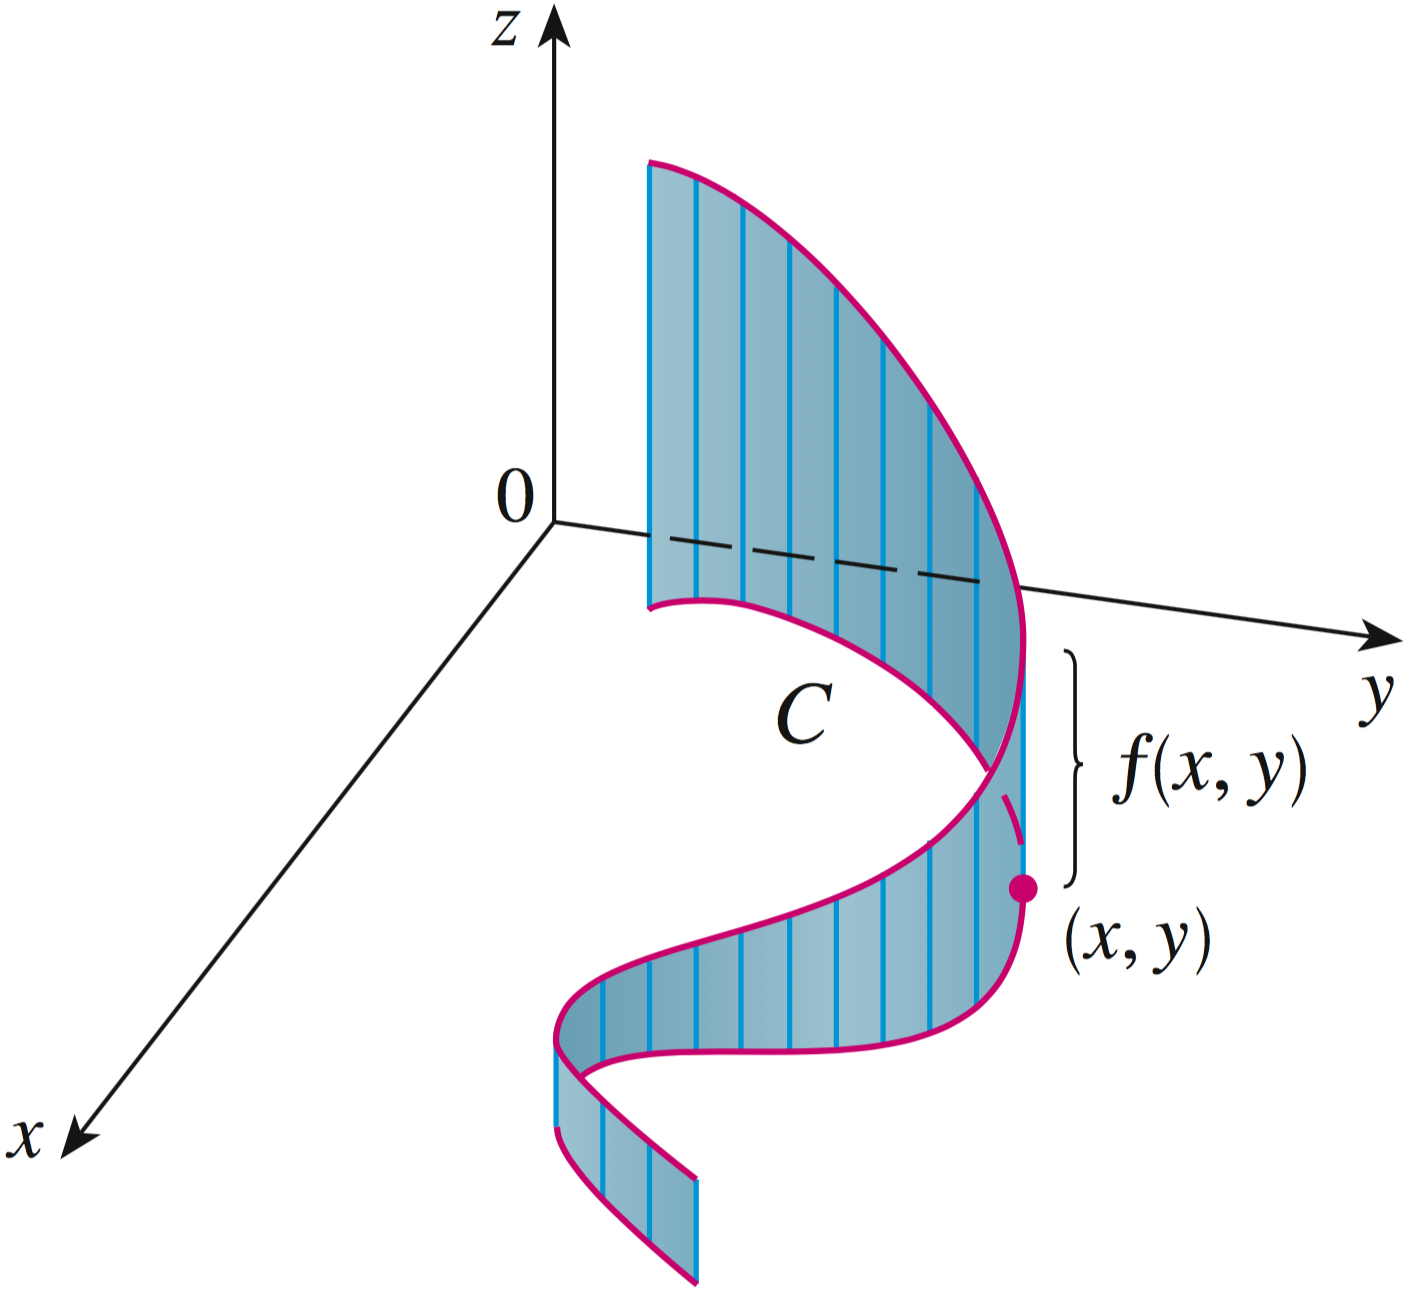
\includegraphics[width=3.5cm]{line_int.png}
        \end{align*}
        \item The value of the line integral does not depend on the parametrization of the curve, provided that the curve is traversed exactly once as $t$ increases from $a$ to $b$.
        \item Just as with single integrals, we can interpret the line integral of a non-negative function as an area.
        \item If $\rho(x,y)$ represents the linear density at a point $(x,y)$ of a wire shaped like a curve $C$, the mass $m$ of the wire is
        \begin{align*}
            m = \int_C \rho(x,y) \,ds
        \end{align*}
        The center of mass of the wire is $(\bar{x}, \bar{y})$ where
        \begin{align*}
            \bar{x} = \frac{1}{m} \int_C x\rho(x,y) \, ds \hspace{5mm} \bar{y} = \frac{1}{m} \int_C y\rho(x,y) \, ds
        \end{align*}
        
        \item Two other line integrals are obtained by replacing $ds$ with $dx$ and $dy$:
        \begin{align*}
            \int_C f(x,y) \,dx = \int_a^b f(x(t), y(t)) \hspace{1mm} x'(t) \,dt \\
            \int_C f(x,y) \,dy = \int_a^b f(x(t), y(t)) \hspace{1mm} y'(t) \,dt 
        \end{align*}
        They are called the line integrals of $f$ along $C$ with respect to $x$ and $y$, respectively. 
        \item If the curve $C$ is a line segment, it is useful to remember the vector representation of a line segment starting at $\vec{r}_0$ and ending at $\vec{r}_1$ is
        \begin{align*}
            \vec{r}(t) = (1-t)\vec{r}_0 + t\vec{r}_1 \hspace{5mm} 0 \leq t \leq 1
        \end{align*}
        
        \item Note that a given parametrization determines an \textbf{orientation} of a curve $C$, with positive direction corresponding to increasing values of $t$. Reversing the orientation has the effect of negating the integral when integrating with respect to $x$ or $y$ (but does not affect the integral when integrating with respect to arc length).
        
        \item \textbf{Line Integrals for space curves:} \\
        Now suppose $C$ is a smooth space curve given by the parametric equations
        \begin{align*}
            x=x(t) \hspace{5mm} y=y(t) \hspace{5mm} z = z(t) \hspace{5mm} a \leq t \leq b
        \end{align*}
        If $f$ is a function of three variables continuous on some region containing $C$, then
        \begin{align*}
            \int_C f(x,y,z) \,ds = \int_a^b f(x(t), y(t),z(t)) \,ds
        \end{align*}
        where 
        \begin{align*}
            ds = \sqrt{ \biggl(\frac{dx}{dt}\biggr)^{\!2} + \biggl(\frac{dy}{dt}\biggr)^{\!2} + 
            \biggl(\frac{dz}{dt}\biggr)^{\!2}} \, dt
        \end{align*}
        % \item If $\vec{r}(t)= \langle x(t), y(t), z(t) \rangle$ is the equivalent vector equation of $C$, observe that the line integral (with respect to arc length) can be written in the more compact vector notation
        % \begin{align*}
        %     \int_a^b f(\vec{r}(t)) \| \vec{r'}(t) \| \, dt
        % \end{align*}
        \item Line integrals along $C$ with respect to $x,y$ or $z$ can also be defined in a similar manner to line integrals in the plane. 
        \item In the case $f(x,y,z)=1$, 
        \begin{align*}
            \int_C  \,ds = L
        \end{align*}
        where $L$ is the length of the curve $C$.
        
        \item \textbf{Line Integrals for vector fields:} \\
        Let $\vec{F}$ be a continuous vector field defined on a smooth curve $C$ given by a vector function $\vec{r}(t), a \leq t \leq b$. The line integral of $\vec{F}$ along $C$ is
        \begin{align*}
            \int_C \vec{F} \cdot d\vec{r} = \int_a^b \vec{F}(\vec{r}(t)) \cdot \vec{r'}(t) \,dt
        \end{align*}
        
        \item Suppose the vector field $\vec{F}=P\vec{i}+Q\vec{j}+R\vec{j}$. We have the following connection between line integrals of vector fields and line integrals of scalar fields:
        \begin{align*}
            \int_C \vec{F} \cdot d\vec{r} = \int_C P \,dx + Q \,dy + R \,dz
        \end{align*}
        \item If $\vec{F}$ is a continuous force field on $\mathbb{R}^3$, such as the gravitational or electric field, we can interpret this integral as the work done by this force in moving a particle along a smooth curve $C$. The work done is negative if the field impedes movement along the curve, and positive otherwise.
    \end{enumerate}
    
    \item \textbf{Fundamental Theorem for Line Integrals}
    \begin{enumerate}
        \item The fundamental theorem of calculus provides a method of evaluating definite integrals by way of a function's anti-derivative. The following theorem can be regarded as a more general version of it for line integrals.
        \item Let $C$ be a smooth curve given by $\vec{r}(t), a \leq t \leq b$. Let $f$ be a differentiable function of two or three variables whose gradient vector $\nabla f$ is continuous on $C$. Then
        \begin{align*}
            \int_C \nabla f \cdot d\vec{r} = f(\vec{r}(b)) - f(\vec{r}(a))
        \end{align*}

        \item We say the line integral $\int_C \vec{F} \cdot d\vec{r}$ is \textbf{independent of path} if $\int_{C_1} \vec{F} \cdot d\vec{r} = \int_{C_2} \vec{F} \cdot d\vec{r}$ for any two paths $C_1$ and $C_2$ that share the same initial and terminal points. 
        \item The theorem implies that line integrals of conservative vector fields are independent of path. Thus we can evaluate the line integral of a conservative vector field simply by knowing the value of a potential function $f$ at the endpoints of $C$.
        \item A curve $C$ is \textbf{closed} if its terminal point coincides with its initial point. A \textbf{simple curve} is a curve that does not intersect itself between endpoints. A \textbf{simply-connected} region $D$ is a connected region $D$ such that every simple closed curve in $D$ encloses only points that are in $D$ (intuitively, this means $D$ is not disjoint and does not contain holes).
        \item $\int_C \vec{F} \cdot d\vec{r}$ is independent of path iff $\int_C \vec{F} \cdot d\vec{r}=0$ for every closed path $C$ in the domain of $\vec{F}$.
        \item In fact, the \textit{only} vector fields that are independent of path are conservative. Suppose $\vec{F}$ is a vector field that is continuous on an open (i.e., does not include boundaries) connected region $D$. If $\int_C \vec{F} \cdot d\vec{r}$ is independent of path in $D$, then $\vec{F}$ is a conservative vector field on $D$.
        % \item Now we consider how to determine if a two-dimensional vector field is conservative (higher dimensions will be explored later).
        \item Let $\vec{F} = P\vec{i} + Q\vec{j}$ be a vector field on an open simply-connected region $D$. If $P$ and $Q$ have continuous first-order partial derivatives and  
        \begin{align*}
            \frac{\partial P}{\partial y} = \frac{\partial Q}{\partial x} 
        \end{align*}
        then $\vec{F}$ is conservative (this follows from Clairaut's theorem).
        \item Suppose we know $\vec{F} = P\vec{i} + Q\vec{j}$ is conservative. To obtain a potential function $f$, we can perform partial integration:
        \begin{align*}
            f(x,y) = \int P(x,y) \,dx \hspace{3mm} \text{or} \hspace{3mm}
            f(x,y) = \int Q(x,y) \,dy
        \end{align*}
        Choose whichever is easier to evaluate. Note that the ``constant of integration" will actually be a function of the opposite variable, $h(y)$ or $h(x)$. Differentiating $f$ with respect to the appropriate variable and comparing the result to $P$ or $Q$ allows us to solve for $h'(y)$ (or $h'(x)$); then partially integrate to obtain $h$.
        \item The method for finding a potential function is much the same for a vector field in $\mathbb{R}^3$. Integrate with respect to $x,y$ or $z$ to obtain $f$; the constant of integration is a function of the other two variables, say $g(y,z)$. Compute $f_y$ and compare with $Q$ to solve for $g_y(y,z)$, then partially integrate with respect to $y$ to obtain $g(y,z)$ (which will involve a constant term $h(z)$). Lastly compute $f_z$ to solve for $h(z)$, as before.
        \item Conservative vector fields appear naturally in physics as they represent forces of physical systems in which energy is conserved (i.e., the sum of kinetic and potential energy is constant).
    \end{enumerate}
    
    \item \textbf{Green's Theorem}
    \begin{enumerate}
        \item Green's theorem gives the relationship between a line integral around a simple closed curve $C$ and a double integral over the plane region $D$ bounded by $C$.
        \item A simple closed curve $C$ has a \textbf{positive orientation} if it is traced out in a counter-clockwise direction. In other words, if $C$ is given by vector function $\vec{r}(t)$, then $D$ is always on the left when we traverse $C$ as $t$ increases.
        \item Let $\vec{F} = P\vec{i} + Q\vec{j}$ be a vector field. Let $C$ be a positively oriented, piecewise smooth, simple, closed curve and let $D$ be the region bounded by $C$. If P and Q have continuous first order partial derivatives on an open region containing $D$, then
        \begin{align*}
            \oint_C P \,dx + Q \,dy = \iint_D \left( \frac{\partial Q}{\partial x} - \frac{\partial P}{\partial y}\right) \, dA
        \end{align*}
        
        \item $\oint_C$ denotes a line integral over a curve $C$ that satisfies the condition of Green’s Theorem.
        \item Green’s Theorem can be used to simplify a line integral over a curve with a lengthy parametrization (e.g., a rectangle). 
        \item An application of Green’s Theorem using the reverse direction is calculating areas. Since the area $A$ of a plane region $D$ is $\iint_D 1 \,dA$, choose $P$ and $Q$ such that $\frac{\partial Q}{\partial x} - \frac{\partial P}{\partial y}=1$. Some possibilities for $(P,Q)$ include $(0,x)$, $(-y,0)$, $(-\frac{1}{2}y, \frac{1}{2}x)$. Thus
        \begin{align*}
            A = \oint_C x \,dy = - \oint y \,dx = \frac{1}{2} \oint_C x \,dy - y \,dx
        \end{align*}
    \end{enumerate}
    
    \item \textbf{Curl and Divergence} 
    \begin{enumerate}
        \item Now we define two operations on vector fields with important applications in physics.
        \item Let $\vec{F} = P\vec{i} + Q\vec{j} + R\vec{k}$ be a vector field on $\mathbb{R}^3$. The \textbf{curl} of $\vec{F}$ is the vector field on $\mathbb{R}^3$ is given by 
        \begin{align*}
            \left( \frac{\partial R}{\partial y} - \frac{\partial Q}{\partial z} \right)\vec{i} + \left( \frac{\partial P}{\partial z} - \frac{\partial R}{\partial x} \right)\vec{j} + \left( \frac{\partial Q}{\partial x} - \frac{\partial P}{\partial y} \right)\vec{k}
        \end{align*}
        
        \item Define the vector differential \textit{operator} $\nabla$ (``del") as
        \vspace{-3mm}
        \begin{align*}
            \nabla = 
            \frac{\partial}{\partial x}\vec{i} + \frac{\partial}{\partial y}\vec{j} + \frac{\partial}{\partial z}\vec{k} 
        \end{align*}
        It operates on a scalar function $f$ to produce the gradient of $f$. Thus we can write
        \begin{align*}
            \text{curl }\vec{F} = 
            \nabla \times \vec{F} =
            \begin{vmatrix}
            \vec{i} & \vec{j} & \vec{k} \\[3 pt]
            \frac{\partial}{\partial x} & \frac{\partial}{\partial y} & \frac{\partial}{\partial z} \\[5 pt]
            P & Q & R
            \end{vmatrix}
        \end{align*}
        % \item It is not hard to verify that the curl of a gradient vector field is $\vec{0}$. Since a conservative vector field is one for which $\vec{F} = \nabla f$, then if $\vec{F}$ is conservative, then $\text{curl }\vec{F}=\vec{0}$. The converse is true if $\vec{F}$ is defined everywhere, and gives the criterion for determining if a vector field on $\mathbb{R}^3$ is conservative.
        \item If $\vec{F}$ is a vector field defined on all of $\mathbb{R}^3$ whose component functions have continuous partial derivatives and $\text{curl }\vec{F}=\vec{0}$, then $\vec{F}$ is a conservative vector field.
        \item If $\vec{F}$ represents the velocity field in fluid flow, then particles near $(x,y,z)$ tend to rotate about the axis that points in the direction of $\text{curl }\vec{F}(x,y,z)$. The magnitude of this vector is a measure of how quickly the particles move about the axis. If $\text{curl }\vec{F}=\vec{0}$ at a point $P$, $\vec{F}$ is called irrotational at $P$.
        \item Let $\vec{F} = P\vec{i} + Q\vec{j} + R\vec{k}$ be a vector field on $\mathbb{R}^3$. The \textbf{divergence} of $\vec{F}$ is the function of three variables defined by
        \begin{align*}
            \text{div }\vec{F} = \frac{\partial P}{\partial x} + \frac{\partial Q}{\partial y} + \frac{\partial R}{\partial z} 
        \end{align*}
        In operator notation, we can write
        \begin{align*}
            \text{div }\vec{F} = \nabla \cdot \vec{F}
        \end{align*}
        \item We have the following relationship between curl and the divergence:
        \begin{align*}
            \text{div curl }\vec{F}=0
        \end{align*}
        \item If $\vec{F}$ represents the velocity field in fluid flow, then $\text{div }\vec{F}(x,y,z)$ is the net rate of change of the mass of the fluid flowing from the point  $(x,y,z)$ per unit volume. If $\text{div }\vec{F}=0$, then $\vec{F}$ is said to be incompressible. If $\text{div }\vec{F}(P)>0$, the net flow is outward near $P$ and $P$ is called a source. If $\text{div }\vec{F}(P)<0$, the net flow is inward near $P$ and $P$ is called a sink. 
        \item Another differential operator arises in computing the divergence of a gradient vector field $\nabla f$. We have
        \begin{align*}
            \text{div } \nabla f = \nabla \cdot (\nabla f) = \frac{\partial^2 f}{\partial x^2} + \frac{\partial^2 f}{\partial y^2} + \frac{\partial^2 f}{\partial z^2} 
        \end{align*}
        The operator $\nabla^2 = \nabla \cdot \nabla$ is called the \textbf{Laplace operator}. Observe that Laplace's equation can be written $\nabla^2 f= 0$.
        \item We can also express Green's theorem in terms of curl and divergence. We have 
        \begin{align*}
            \oint_C \vec{F} \cdot \,d\vec{r} = \iint_D (\text{curl }\vec{F}) \cdot \vec{k} \,dA
        \end{align*}
        where $\vec{k}$ is the standard unit vector in the $z$ direction. 
        \item If the curve $C$ is given by the vector equation $\vec{r}(t)=x(t)\vec{i} + y(t)\vec{j}$, $a \leq t \leq b$, the outward unit normal vector to $C$ is given by
        \begin{align*}
            \vec{n}(t) = \frac{y'(t)}{\| \vec{r'}(t) \|}\vec{i} - \frac{x'(t)}{\| \vec{r'}(t) \|}\vec{j}
        \end{align*}
        We have
        \begin{align*}
            \oint_C \vec{F} \cdot \vec{n} \,ds = \iint_D \text{div }\vec{F}(x,y) \,dA
        \end{align*} 
    \end{enumerate}
    \item \textbf{Parametric Surfaces}
    \begin{enumerate}
        \item In much the same way we describe a space curve by a vector function $\vec{r}(t)$ of $t$, we can describe a surface by a vector function $\vec{r}(u,v)$ of $u$ and $v$.
        \item Suppose $\vec{r}(u,v) = \langle x(u,v), y(u,v), z(u,v) \rangle$ is a vector-valued function on a region $D$ in the $uv$-plane. The set of all points $(x,y,z)$ such that $\vec{r}(u,v) = \langle x,y,z \rangle$ as $(u,v)$ varies throughout $D$ is called a \textbf{parametric surface}.
        \item Setting $u$ or $v$ constant in the vector function $\vec{r}(u,v)$ correspond to vertical and horizontal lines in the $uv$-plane and are called \textbf{grid curves}.
        
        \item The ellipsoid $ax^2 + by^2 + cz^2 = d^2$ can be parametrized as $$\vec{r}(\phi, \theta) = \left< \frac{d}{\sqrt{a}}\sin{\phi}\cos{\theta}, \frac{d}{\sqrt{b}}\sin{\phi}\sin{\theta}, \frac{d}{\sqrt{c}}\cos{\phi} \right>$$ for $0 \leq \phi \leq \pi$ and $0 \leq \theta \leq 2\pi$.
        \item A surface given as the graph of a function $z=f(x,y)$ can always be regarded as a parametric surface by taking $x$ and $y$ as parameters and writing the parametric equation for $z$ as $z=f(x,y)$.
        \item The surface obtained by rotating the curve $y=f(x)$, $a \leq x \leq b$, $f(x) \geq 0$ about the $x$-axis can be parametrized by $x=x$, $y=f(x)\cos{\theta}$, $z=f(x)\sin{\theta}$ for $a \leq x \leq b$, $0 \leq \theta \leq 2\pi$.
        \item Let $S$ be the surface traced out by vector function $\vec{r}(u,v)$. Let $\vec{r}_u$ and $\vec{r}_v$ denote the partial derivatives of $\vec{r}(u,v)$ with respect to $u$ and $v$, respectively (which are vector-valued functions). If $\vec{r}_u \times \vec{r}_v \neq \vec{0}$ (i.e., $S$ is smooth), $\vec{r}_u \times \vec{r}_v$ is a normal vector to the tangent plane to $S$.
        \item If a smooth parametric surface $S$ is given by vector equation $\vec{r}(u,v)$ for $(u,v) \in D$ and $S$ is covered just once as $(u,v)$ ranges throughout the parameter domain $D$, then the \textbf{surface area} of $S$ is
        \begin{align*}
            SA = \iint_D \| \vec{r}_u \times \vec{r}_v \| \,dA
        \end{align*}
        \item In the special case of a surface $S$ with equation $z=f(x,y)$ for $(x,y) \in D$, the surface area formula becomes
        \begin{align*}
            SA = \iint_D \sqrt{1 + \biggl( \frac{\partial z}{\partial x} \biggr)^2 + \biggl( \frac{\partial z}{\partial y} \biggr)^2} \,dA
        \end{align*}
    \end{enumerate}
    
    \item \textbf{Surface Integrals}
    \begin{enumerate}
        \item Surface integrals are the double integral analog of the line integral; we integrate a function of three variables along a surface.
        \item If a smooth parametric surface $S$ is given by vector equation $\vec{r}(u,v)$ for $(u,v) \in D$ and $S$ is covered just once as $(u,v)$ ranges throughout the parameter domain $D$, the \textbf{surface integral} of $f$ over the surface $S$ is
        \begin{align*}
            \iint_S f(x,y,z) \,dS = \iint_D f(\vec{r}(u,v)) \| \vec{r}_u \times \vec{r}_v \| \,dA
        \end{align*}
        \item Observe that in the case $f(x,y,z)=1$, $\iint_D \,dS$ is the surface area of $S$.
        \item If a thin sheet with density function $\rho(x,y,z)$ has the shape of a surface $S$, the mass of the sheet is
        \begin{align*}
            m = \iint_S \rho(x,y,z) \,dS
        \end{align*}
        The center of mass is $(\bar{x}, \bar{y}, \bar{z})$, where
        \begin{align*}
            \bar{x} = \frac{1}{m} \iint_S x\rho(x,y,z) \,dS 
        \end{align*}
        with $\bar{y}$ and $\bar{z}$ defined similarly.
        
        \item In the case $S$ is a surface with equation $z=g(x,y)$, this formula becomes
        \begin{align*}
            &\iint_S f(x,y,z) \,dS  \\ &=\iint_D f(x,y,g(x,y)) \sqrt{1 + \biggl( \frac{\partial z}{\partial x} \biggr)^2 + \biggl( \frac{\partial z}{\partial y} \biggr)^2} \,dA
        \end{align*}
        Similar formulas apply if it is more convenient to express $S$ as a function of $y$ and $z$ or $x$ and $z$. 
        
        \item \textbf{Surface Integrals for vector fields} \\
        An \textbf{orientable} surface $S$ is two-sided (distinction is needed as a Mobius strip is one-sided). If it is possible to choose a unit normal vector $\vec{n}$ at every point $(x,y,z)$ so that $\vec{n}$ varies continuously over $S$, then $S$ is called an \textbf{oriented surface}. The choice of $\vec{n}$ provides $S$ with an \textbf{orientation}; there are two possible orientations from using $\vec{n}_1$ or $\vec{n}_2 = - \vec{n}_1$. 
        \item For a closed surface, that is, a surface that is the boundary of a solid region $E$, the \textbf{positive orientation} is the one for which the normal vectors point outward from $E$, and inward-pointing normals give the \textbf{negative orientation}.
        \item If $\vec{F}$ is a continuous vector field defined on an oriented surface $S$ with unit normal vector $\vec{n}$, then the surface integral of $\vec{F}$ over $S$ is
        \begin{align*}
            \iint_S \vec{F} \cdot d\vec{S} = \iint_S \vec{F} \cdot \vec{n} \,dS
        \end{align*}
        This integral is also called the \textbf{flux} of $\vec{F}$ across $S$.
        \item If $S$ is given by vector function $\vec{r}(u,v)$, we have
        \begin{align*}
            \iint_S \vec{F} \cdot d\vec{S} = \iint_D \vec{F} \cdot (\vec{r}_u \times \vec{r}_v) \,dA
        \end{align*}
        In the case $S$ is given by the graph $z=g(x,y)$, then
        \begin{align*}
            \iint_S \vec{F} \cdot d\vec{S} = \iint_D \left( -P\frac{\partial g}{\partial x} - Q \frac{\partial g}{\partial y} + R \right) \,dA
        \end{align*}
        which assumes the upward orientation of $S$; for the downward orientation multiply the integrand by $-1$. Similar formulas apply if $S$ is given by $y=h(x,z)$ or $x=k(y,z)$.
        \item If $\vec{F}$ is a velocity field, the surface integral can be interpreted as the flow rate of fluid through $S$. Over an electric field, the surface integral is called the electric flux. By Gauss's Law, the net charge enclosed by a closed surface $S$ in an electric field $\vec{E}$ is
        \begin{align*}
            Q = \epsilon_0 \iint_S \vec{E} \cdot d\vec{S}
        \end{align*}
        where $\epsilon_0$ is the permittivity of free space.
    \end{enumerate}
    
    \item \textbf{Stokes' Theorem}
    \begin{enumerate}
        \item Stokes' Theorem is a higher-dimensional version of Green's Theorem. It relates a surface integral over a surface $S$ to a line integral around the boundary curve of $S$.
        \item Let $S$ be an oriented piecewise-smooth surface that is bounded by a simple, closed, smooth boundary curve $C$ with positive orientation. Let $\vec{F}$ be a vector field whose components have continuous partial deriviatives on an open region in $\mathbb{R}^3$ that contains $S$. Then
        \begin{align*}
            \int_C \vec{F} \cdot d\vec{r} = \iint_S \text{curl } \vec{F} \cdot d\vec{S}
        \end{align*}
        Note that the positively oriented boundary curve of $S$ is often written as $\partial S$ instead of $C$.
        
        \item In the special case where $S$ is flat and lies in the $xy$-plane with upward  orientation, the unit normal vector is $\vec{k}$, the surface integral becomes a double integral, and Stokes' Theorem becomes the curl vector version of Green's Theorem given earlier.
    \end{enumerate}
    
    \item \textbf{The Divergence Theorem}
    \begin{enumerate}
        \item Let $E$ be a simple solid region (i.e., $E$ is simultaneously type 1, 2, and 3) and let $S$ be the boundary surface of $E$ with positive outward orientation. Let $\vec{F}$ be a vector field whose component functions have continuous partial derivatives. Then
        \begin{align*}
            \iint_S \vec{F} \cdot d\vec{S} = \iiint_E \text{div } \vec{F} \,dV
        \end{align*}
        So the flux of $\vec{F}$ across the boundary surface of $E$ is equal to the triple integral of the divergence of $\vec{F}$ over $E$.
        \item In practice, this theorem is useful for converting a difficult surface integral into a simpler triple integral.
    \end{enumerate}
\end{enumerate}
\end{multicols}


%~~~~~~~~~~~~~APPENDIX~~~~~~~~~~~~~

\newpage
\begin{multicols}{2}
\section{Single Variable Calculus Appendix}
\begin{enumerate}
    \item \textbf{Trigonometry}
    \begin{enumerate}
        \item     
        \begin{align*}
        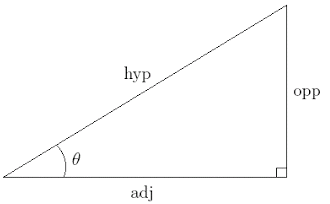
\includegraphics[width=3cm]{tri.png}
        \end{align*}
        \begin{align*}
        \hspace{-8mm}
            \sin{\theta} = \frac{\text{opp}}{\text{hyp}} \hspace{6mm}
            \cos{\theta} = \frac{\text{adj}}{\text{hyp}} \hspace{6mm}
            \tan{\theta} = \frac{\text{opp}}{\text{adj}} 
        \end{align*}
        
        \item 
        \begin{tabular}[t]{lll}
        $\sin{0} = 0$ & $\cos{0} = 1$ & $\tan{0} = 0$ \\[6pt]
        $\sin{\frac{\pi}{6}} = \frac{1}{2}$ & $\cos{\frac{\pi}{6}} = \frac{\sqrt{3}}{2}$ & $\tan{\frac{\pi}{6}} = \frac{1}{\sqrt{3}}$ \\[6pt]
        $\sin{\frac{\pi}{4}} = \frac{\sqrt{2}}{2}$ & $\cos{\frac{\pi}{4}} = \frac{\sqrt{2}}{2}$ & $\tan{\frac{\pi}{4}} = 1$ \\[6pt]
        $\sin{\frac{\pi}{3}} = \frac{\sqrt{3}}{2}$ & $\cos{\frac{\pi}{3}} = \frac{1}{2}$ & $\tan{\frac{\pi}{3}} = \sqrt{3}$ \\[6pt]
        $\sin{\frac{\pi}{2}} = 1$ & $\cos{\frac{\pi}{2}} = 0$ & $\tan{\frac{\pi}{2}} = \infty$ \\
        \end{tabular} 

        \item     
        \begin{align*}
            \sin^2{\theta} + \cos^2{\theta} = 1 \hspace{10mm} & \sin{2\theta} = 2\sin{\theta}\cos{\theta} \\
            1 + \tan^2{\theta} = \sec^2{\theta} \hspace{10mm} & \cos{2\theta} = \cos^2{\theta} - \sin^2{\theta} \\
            1 + \cot^2{\theta} = \csc^2{\theta} \hspace{10mm} & \hspace{9.4mm} = 2\cos^2{\theta} - 1 \\
         \hspace{10mm} & \hspace{9.4mm} = 1 - 2\sin^2{\theta} 
        \end{align*}
        
        
        \item     
        \begin{align*}
            \sin^2{\theta} = \frac{1-\cos{2\theta}}{2} & \hspace{10mm} \sin{-\theta} = -\sin{\theta} \\
            \cos^2{\theta} = \frac{1 + \cos{2\theta}}{2} & \hspace{10mm} \cos{-\theta} = \cos{\theta} \\
            \tan^2{\theta} = \frac{1-\cos{2\theta}}{1+\cos{2\theta}} & \hspace{10mm} \tan{-\theta} = -\tan{\theta} 
        \end{align*}

        \item 
        \begin{align*}
            \sin{\alpha + \beta} = \sin{\alpha}\cos{\beta} + \sin{\beta}\cos{\alpha} \\
            \cos{\alpha + \beta} = \cos{\alpha}\cos{\beta} - \sin{\alpha}\sin{\beta} 
        \end{align*}
    \end{enumerate}
    
    \item \textbf{Derivatives} 
    \begin{enumerate}
        \item Product Rule: $(f(x)g(x))' = f'(x)g(x) + f(x)g'(x)$
        \item Quotient Rule: $ \left( \frac{f(x)}{g(x)} \right)' = \frac{f'(x)g(x) - f(x)g'(x)}{g(x)^2}$
        \item Chain Rule: $ (f (g (x)))' = f'(g(x))g'(x)$
        \item A function is convex if $f''(x) > 0$ and concave if $f''(x) < 0$.
        \item Implicit Differentiation: $y$ is defined \textit{implicitly} as a function of $x$. Differentiate both sides of the equation with respect to $x$; $y$ becomes $\frac{dy}{dx}$.
        \item
        \begin{tabular}[t]{ll}
        $\frac{d}{dx}(ax^n) = nax^{n-1}$                        & $\frac{d}{dx}(\sin{x}) =  \cos{x}$   \\[6pt]
        $\frac{d}{dx}(a^x) = a^x \ln{a}$                        & $\frac{d}{dx}(\cos{x}) = -\sin{x}$   \\[6pt]
        $\frac{d}{dx}(\ln{x}) = \frac{1}{x}$                    & $\frac{d}{dx}(\tan{x}) =  \sec^2{x}$ \\[6pt]
        $\frac{d}{dx}(\log_a{x}) = \frac{1}{x\ln{a}}$           & $\frac{d}{dx}(\sin^{-1}{x}) = \frac{1}{\sqrt{1-x^2}}$ \\[6pt]
        $\frac{d}{dx}(\cos^{-1}{x}) = -\frac{1}{\sqrt{1-x^2}}$  & $\frac{d}{dx}(\tan^{-1}{x}) = \frac{1}{1+x^2}$ \\[6pt]
        \end{tabular}

    \end{enumerate}
    \item \textbf{Integrals}
    \begin{enumerate}
    \item 
    \begin{tabular}[t]{lll}
    $\int a \, dx = ax + c$      					& $\int e^x \, dx = e^x + c$            \\[6pt]
    $\int x^n \, dx = \frac{1}{n+1}x^{n+1} + c$     & $\int \sin{x} \, dx = -\cos{x} + c$   \\[6pt]     
    $\int \frac{1}{x} \, dx = \ln{|x|} + c$      	& $\int \cos{x} \, dx = \sin{x} + c$    \\[6pt]     
    $\int \ln{x} \, dx = -x + x\ln{x} + c$          & $\int \sec^2{x} \, dx = \tan{x} + c$  \\[6pt]
    \end{tabular}
    
    
    \item Arc length: The arc length of a curve of the form $y=f(x)$, $a \leq x \leq b$ is given by 
    \begin{align*}
        L = \int_a^b \sqrt{1 + \left(\frac{dy}{dx}\right)^2} \, dx
    \end{align*}
    \item U-Substitution: To compute $\int f(g(x))g'(x) \, dx$, let $u=g(x)$ and $du = g'(x) \, dx$. Then $$\int f(g(x))g'(x) \, dx = \int f(u) \, du$$
    Compute the anti-derivative and then re-substitute $u$.
    
    \item Integration by Parts: 
    \begin{align*}
        \int_a^b u \, dv = [uv]_a^b - \int_a^b v \, du
    \end{align*}
    \end{enumerate}
    
    \item \textbf{Miscellaneous}
    \begin{enumerate}
        \item L’Hospital’s rule:
        If we have 
        \begin{align*}
            \lim_{x \rightarrow a} \frac{f(x)}{g(x)} = \frac{0}{0} \text{ or } \frac{\pm\infty}{\pm\infty}
        \end{align*}
        then 
        \begin{align*}
            \lim_{x \rightarrow a} \frac{f(x)}{g(x)} = \lim_{x \rightarrow a} \frac{f'(x)}{g'(x)}
        \end{align*}
        \item Completing the square: 
        \begin{align*}
            x^2 + bx = 0 &\rightarrow x^2 + bx + \left(\frac{b}{2}\right)^2 = \left(\frac{b}{2}\right)^2 \\ & \rightarrow \left(x+\frac{b}{2}\right)^2 = \left(\frac{b}{2}\right)^2
        \end{align*}
    \end{enumerate}
\end{enumerate}
\end{multicols}
\end{document}